% !TEX root = laplace_beltrami.tex

%%%%%%%%%%%%%%%%%%%%%%%%%%%%%%%%%%%%%%%%%%%%%%%%%%%%%%%%%%%%%%%%%%%%%%%%%%%%%%%%
\section{Parametric Finite Element Method}\label{sec:parametric}
%%%%%%%%%%%%%%%%%%%%%%%%%%%%%%%%%%%%%%%%%%%%%%%%%%%%%%%%%%%%%%%%%%%%%%%%%%%%%%%%

The parametric method hinges on a surface approximation $\Gamma$
``interpolating'' the exact surface $\gamma$.
Recall that the latter is assumed to be a closed, compact, orientable hypersurface in $\mathbb R^{n+1}$.
In the lowest order case of piecewise linear polynomials, this corresponds to a polyhedral surface $\Gamma$ whose vertices lie on $\gamma$ or, more generally, sufficiently close to $\gamma$.  The finite element space is then obtained in a classical way by mapping a finite element triplet defined on a reference element in $\mathbb R^n$ to a facet of $\Gamma$ in $\mathbb R^{n+1}$. The FEM requires a bi-Lipschitz map $\bP:\Gamma\to\gamma$ which is not necessarily the distance function lift $\bP_d$. The latter is used for numerical analysis purposes only even for smooth surfaces.

There are two sources of error: the approximation of the exact surface $\gamma$ by the polyhedral surface $\Gamma$, the so-called \emph{geometric consistency error}, and the \emph{Galerkin error} arising from the actual finite element approximation on $\Gamma$. In this section we quantify these two errors depending on the regularity of $\gamma$.
For the former we rely on the discussion of section \ref{S:perturbation} that addresses
the effect of perturbing $\gamma$.
For $\gamma$ of class $C^{1,\alpha}$ we deal with
a generic lift $\bP:\Gamma\to\gamma$ and
obtain a suboptimal geometric consistency error.
For $C^2$ surfaces, instead, we resort to $\bP_d$
for error analysis and restore geometric optimality.


%-------------------------------------------------------------------------------
\subsection{FEM on Lipschitz Parametric Surfaces.}
%-------------------------------------------------------------------------------

%-------------------------------------------------------------------------------
\noindent
{\bf Lipschitz Parametric Surfaces.}
%-------------------------------------------------------------------------------
We adopt the viewpoint that the surface $\gamma$ is described as the deformation of an
$n$-dimensional polyhedral surface $\lingamma$ by a globally bi-Lipschitz
\emph{homeomorphism} $\bP:\lingamma \rightarrow \gamma \subset \mathbb
R^{n+1}$. 
Thus there exists $L>0$ such that for all $\bx_1, \bx_2 \in \lingamma$
\begin{equation}
\label{surf_bi_lipschitz}
L^{-1} |\bx_1-\bx_2| \le |\widetilde{\bx}_1 -\widetilde{\bx}_2| \le L|\bx_1-\bx_2|, \qquad
\widetilde{\bx}_i = \bP(\bx_i), ~i=1,2.
\end{equation}
If $\gamma$ is $C^2$, we may take $\bP=\bP_d$, but our current definition allows for much more flexibility in the choice of $\bP$.  For example, if $\gamma$ has nonempty boundary and is given as the graph of a function $\psi:\Omega \rightarrow \mathbb{R}^{n+1}$ with $\Omega \subset \mathbb{R}^n$, then the map between $\bx=(x,z) \in \Gamma$ with $x \in \Omega$ and $z \in \mathbb{R}$ could be given by $\bP(x,z)=(x, \psi(x))\in\gamma$, i.e., the ``vertical'' graph map.  

The (closed) facets of $\lingamma$ are denoted by $T$, and form the collection $\T=\{T \}$.   We assume that these facets are all simplices and denote by $S_\T$ the set of interior faces of $\T$.  Extension to other element shapes such as $n$-quadrilaterals and to nonconforming discretizations is possible under reasonable assumptions with minor modifications, but we do not elaborate them further.  
We let $\bP_T:T \rightarrow \mathbb R^{n+1}$ be
the restriction of $\bP$ to $T$.
The partition $\T$ of $\lingamma$ induces the partition
$\widetilde{\T}=\{\widetilde{T}\}_{T \in \T}$ of $\gamma$ upon setting
%
\[
\widetilde{T} := \bP_T(T)
\quad\forall \, T\in \T.
\]
Note that this \emph{non-overlapping} parametrization of $\gamma$ allows for Lipschitz surfaces rougher than globally $C^2$.  We additionally define {\it macro patches} 
%
\begin{equation}\label{patch}
\linpatch_T=\cup \big\{T': T' \cap T \neq \emptyset \big\},
\qquad
\widetilde{\omega}_T =  \bP(\linpatch_T).
\end{equation}
%
Let $h_T := | T |^{\frac 1 n}$ and
$\sigma < \infty$ be the triangulation shape-regularity constant, i.e.
%
\begin{equation}\label{e:shape_reg}
\sigma:=\sup_{\T} \max_{T \in \T} \frac{{\rm diam}(T)}{h_T}.
\end{equation}
%
We further assume that the number of elements in each patch $\omega_T$ is uniformly bounded.  This assumption automatically follows from shape regularity for triangulations of Euclidean domains, but the situation is more subtle for surface triangulations as illustrated in Figure~\ref{f:valence}.  Such a bound does for example hold if $\lingamma$ is obtained by systematic refinement of an initial surface mesh with a uniform bound on the number of elements in a patch \cite{DemlowDziuk:07}, or more generally using adaptive refinement strategies \cite{BCMMN16,BCMN:Magenes}.  In addition, this implies that all elements in $\linpatch_T$ have uniformly equivalent diameters, as it happens for shape regular triangulations on Euclidean domains.

%
\begin{figure}[ht!]
\centerline{\includegraphics[width=0.5\textwidth]{shape_n12}
\includegraphics[width=0.5\textwidth]{shape_n22}}
\caption{
Two different configurations when $n=2$ illustrating that the number of elements sharing the same vertex could be arbitrarily large even when using triangles satisfying \eqref{e:shape_reg_init}.} \label{f:valence}
\end{figure}

To provide a parametric description,
let $\widehat{T}$ be the unit reference simplex, sometimes called the {\it universal parametric domain}.
We denote by $\linparam_T:\mathbb R^n\to\mathbb R^{n+1}$ the affine map such that $T = \linparam_T(\widehat{T})$ and note that \eqref{e:shape_reg} implies
%
\begin{equation}\label{e:shape_reg_init}
h_T | \bw|  \lesssim | D \linparam_T \bw | \lesssim h_T | \bw|, \qquad \forall \bw \in \mathbb R^n. 
\end{equation}
Hereafter we omit to specify when the constants (possibly hidden in $\lesssim$ signs) depend on $\sigma$.
As pointed out in \cite{BP:11}, even if the initial surface approximation satisfies \eqref{e:shape_reg_init}, this property might not hold for refinements unless the initial polyhedral surface approximates the exact surface well. 
We refer to \cite{BCMMN16,BCMN:Magenes} for a discussion on how to circumvent this in an adaptive strategy.
However, since this work focusses on a-priori and a-posteriori error estimation rather that adaptivity, we assume \eqref{e:shape_reg_init} directly. 
%

We are now ready to introduce the local {\it non-overlapping} parametrization $\bchi$
of $\gamma$.
Let $\exactparam_T := \bP \circ\linparam_T: \widehat{T} \rightarrow \widetilde{T}$ be the corresponding local parametrization of $\widetilde{T}$ and $\bchi:= \{ \bchi_T \}_{T\in \T}$; see Figure~\ref{f:param}.
We record for latter use that thanks to the Lipschitz properties \eqref{surf_bi_lipschitz} and \eqref{e:shape_reg_init}, $\exactparam_T$ also satisfies 
\begin{equation}\label{e:shape_reg_exact}
  h_T | \bw|  \lesssim | D \exactparam_T(\by) \bw | \lesssim h_T | \bw |
 \quad \forall \bw \in \mathbb R^n, ~ \by\in\widehat{T}.
\end{equation}
%
\begin{figure}[ht!]
\begin{picture}(0,0)
\put(-75,-140){$\widehat T$}
\put(10,-120){$\linparam_T$}
\put(30,-65){$T\subset \Gamma$}
\put(15,-50){$\bP$}
\put(30,5){$\widetilde T \subset \gamma$}
\put(-40,-75){$\exactparam_T$}
\end{picture}
\centerline{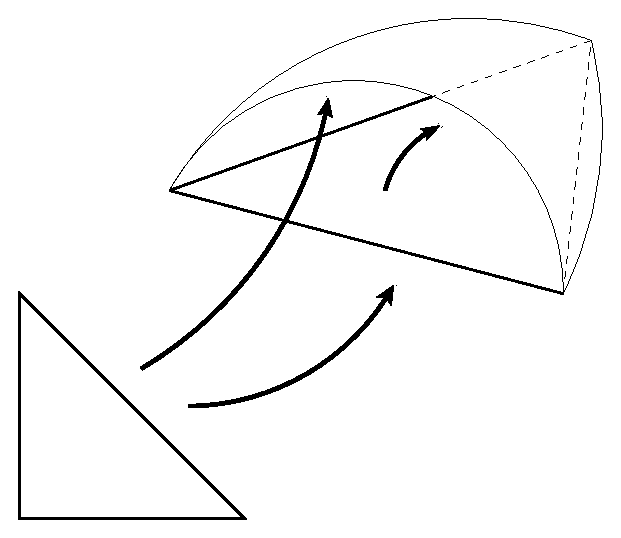
\includegraphics[width=0.5\textwidth]{parametric}}
\caption{
Non-overlapping parametrizations  $\linparam_T : \widehat T \rightarrow T$ of $\Gamma$ and $\exactparam_T : \widehat T \rightarrow \widetilde T$ of $\gamma$.} \label{f:param}
\end{figure}

It turns out that it
will be convenient to consider $\bchi_T$ to be defined on a larger domain than $T$,
say $\widehat{\omega}_T\subset\mathbb{R}^n$, so that 
$\exactparam_T = \bP \circ\linparam_T:\widehat{\omega}_T \to\widetilde{\omega}_T$
is a  bi-Lipschitz local parametrization of $\gamma$: there exists
a universal constant $L\geq1$ such that for each fixed $T \in \T$ and
for all $\widetilde \bx_1=\exactparam_T(\by_1), \widetilde \bx_2=\exactparam_T(\by_2)
\in \widetilde{\omega}_T$, 
%
\begin{equation}\label{bi_lipschitz}
L^{-1} h_T  |\by_1-\by_2| 
\le |\widetilde \bx_1 -  \widetilde \bx_2 | 
\le L h_T |\by_1-\by_2|;
\end{equation}
%
in this case $\bchi:= \{ \bchi_T \}_{T\in \T}$ is an {\it overlapping} parametrization
of $\gamma$.
We further assume that $\bP(\mathbf v) = \mathbf v$ 
for all vertices $\mathbf v$ of $\lingamma$, so that $\linparam_T$ is the nodal
Lagrange interpolant of $\exactparam_T$ into linears.  

We finally note that a function $\widetilde \tv_T:\widetilde{T}\to\mathbb R$ defines uniquely two
functions $\widehat{\tv}_T:\widehat{T}\to\mathbb R$ and $\tv_T:T\to\mathbb R$ via the
maps $\bXi_T$ and $\bP$, namely
%
\begin{align}  \label{para_lift}
\widehat{\tv}_T(\by) := \widetilde \tv_T(\exactparam_T(\by)) \quad \forall\; \widehat{\bx}\in
\widehat{T} \quad \text{ and }\quad \tv_T(\bx) := \widetilde \tv_T(\bP(\bx))
\quad\forall\; \bx\in T.
\end{align}
%
Moreover, each one of these functions induces the other two uniquely. Accordingly,
we will use the symbol $\tv$ for all three functions if no confusion arises.


%--------------------------------------------------------------------------------
\medskip\noindent
{\bf Differential Geometry on Polyhedral Surfaces.} %\label{S:diff-geom}
%--------------------------------------------------------------------------------
%
We use the  atlas $\{\widehat{T},\widetilde{T},\bchi_T\}_{T\in\T}$,
induced by the non-overlapping parametrization $\bchi:= \{ \bchi_T \}_{T\in \T}$,
to describe $\gamma$ in the spirit of Section \ref{sec:preliminaries}.
Likewise, we employ the atlas $\{\widehat{T},T,\bX_T\}_{T\in\T}$ to describe
the polyhedral surface $\Gamma$.
In view of \eqref{e:shape_reg_exact}, 
the discrete first fundamental form $\bg_T$ and area element $q_T$ of $\Gamma$
are given elementwise by
%
\begin{equation}\label{area}
  \bg_T := (D \bX_T)^t D \bX_T,
  \quad
  q_T := \sqrt{\det\bg_T},
  \quad\forall \, T\in\T.
\end{equation}
%
and satisfy
%
\begin{equation}\label{e:eigen_g}
  \textrm{eigen}(\bg_T) \approx h_T^2, \quad  q_T \approx h_T^n,
  \quad\forall \, T\in\T.
\end{equation}
%
They give rise to the piecewise constant functions $\bg_\Gamma:=\{\bg_T\}_{T\in\T}$
and $q_\Gamma:=\{q_T\}_{T\in\T}$. Similar properties are enjoyed by $\bchi$, which
imply that the stability constant $S_\bchi$ defined in \eqref{stab-const} is purely
geometric and independent of meshsize:
%
\begin{equation}\label{Sapprox1}
S_\bchi \approx 1.
\end{equation}
%
In addition, notice that \eqref{e:shape_reg_exact} and \eqref{bi_lipschitz} imply that
\begin{equation}\label{q:nondegen:assume}
C_1 \le \frac{q}{q_\Gamma} \le C_2
\end{equation}
for constants $C_1$, $C_2$ independent of discretization parameters.
%
Moreover, the
vector $\bN_T := \sum_{i=1}^{n+1} \det\big([\be_j, D \bX_T)]\big) \be_j$
is perpendicular to $T\in\T$
provided $\{ \be_j \}_{j=1}^{n+1}$ are the canonical unit vectors of $\mathbb R^{n+1}$.
This vector satisfies $|\bN_T|=q_T$ and yields the unit normal to $T$
%
\[
\bnu_T := \frac{\bN_T}{|\bN_T|}
\quad\forall \, T\in\T,
\]
%
and corresponding piecewise constant unit normal vector
$\bnu_\Gamma := \{ \bnu_T \}_{T \in \T}$ to $\Gamma$.

Given a function $\tv:\Gamma\to\mathbb{R}$, its tangential gradient
$\nabla_\Gamma\tv$ and Laplace-Beltrami operator $\Delta_\Gamma \tv$ over $\Gamma$
obey the formulas
%
\begin{equation}\label{grad-Gamma}
  \nabla \widehat\tv = (D \bX)^t \, \nabla_{\Gamma} \tv, \quad
  \nabla_{\Gamma} \tv = (D \bX) \, \bg_\Gamma^{-1} \, \nabla \widehat\tv,
\end{equation}
and 
\begin{equation}\label{lap-bel}
\Delta_\Gamma \tv = \frac{1}{q_\Gamma} {\text{div}} 
\big(q_\Gamma  \, \bg_\Gamma^{-1} \, \nabla\widehat\tv \big),
\end{equation}
%
where $\widehat \tv:{\widehat{T}}\to\mathbb{R}$ is defined in \eqref{para_lift}.
The strong form of $\Delta_\Gamma \tv$ is well defined only elementwise because
$q_\Gamma  \, \bg_\Gamma^{-1}$ is piecewise constant and so discontinuous over $\T$.
To find the correct strong form we start from the weak form \eqref{e:weak_relax},
split the integral over elements and use Corollary \ref{C:int-parts}
(integration by parts) to obtain
%
\begin{align*}
  \int_\Gamma \nabla_\Gamma \tv \cdot \nabla_\Gamma w & =
  \sum_{T\in\T} -\int_T w \Delta_\Gamma \tv +
  \int_{\partial T} w \nabla_\Gamma\tv\cdot\bmu_T
  \\
  & = \sum_{T\in\T} -\int_T w \Delta_\Gamma \tv +
  \sum_{S\in\mathcal{S}} \int_S w [\nabla_\Gamma \tv],
\end{align*}
%
where the jump residual is computed over each face $S\in\mathcal{S}$ of elements of $\T$
via
%
\begin{equation}\label{jump-residual}
  [\nabla_\Gamma v] := \nabla_\Gamma \tv_+ \cdot \bmu_+
    + \nabla_\Gamma \tv_- \cdot \bmu_-
\end{equation}
%
and $T_\pm \in\T$ are such that $S=T_+ \cap T_-$ and $\tv_\pm, \bmu_\pm$ are the
restrictions of $\tv$ and the outer unit normal to $\partial T_\pm$ which is parallel
to $T_\pm$. We then see that $\Delta_\Gamma \tv$ consists of the absolutely
continuous part \eqref{lap-bel} with respect to surface measure defined elementwise
and the singular part \eqref{jump-residual} supported on the skeleton of $\T$. This
formula makes sense for functions which are piecewise $H^2$ and globally $H^1$, such
as continuous piecewise polynomials.


%-------------------------------------------------------------------------------
\medskip\noindent
{\bf Parametric Finite Element Method.} %\label{ss:fem}
%-------------------------------------------------------------------------------
%
In this work, we focus on continuous piecewise linear finite elements and
polyhedral surface approximations.
Let $\mathcal P$ be the space of linear polynomials and let $\V(\T)$ be the
space of continuous piecewise linear polynomial functions over $\Gamma$, namely
%
\begin{equation*}
\V(\T) :=\left\lbrace V \in C^0(\Gamma)  \;\big|\; 
	   V|_{T}  = \widehat V \circ \bX^{-1} \mbox{ for some } \widehat V\in \mathcal P, ~T \in \T\right\rbrace.
\end{equation*}
%
The finite element space associated with the Laplace-Beltrami equation over
$\Gamma$ is the restriction of $\V(\T)$ to functions with vanishing mean
%
\[
\V_\#(\T):= \V(\T) \cap L_{2,\#}(\Gamma).
\]
%
We define $\interp: C^0(\Gamma) \to \V(\T)$ to be the Lagrange interpolation operator
and use the same notation for vector-valued functions.

We are now ready to introduce the parametric FEM: seek $U:=U_\T \in \V_\#(\T)$
that solves
%o
\begin{equation}\label{e:galerkin}
  \int_\Gamma \nabla_\Gamma U \cdot \nabla_\Gamma V = \int_\Gamma F V
  \quad \forall V \in \V_\#(\T),
\end{equation}
where $F \in L_{2,\#}(\Gamma)$ is an approximation of $f \in L_{2,\#}(\gamma)$ to be specified later.
Lax-Milgram theory guarantees that $U \in \V_\#(\T)$ is well defined. 
Observe that because $F \in L_{2,\#}(\Gamma)$, we also have
\begin{equation}\label{e:galerkin_relax}
  \int_\Gamma \nabla_\Gamma U \cdot \nabla_\Gamma V = \int_\Gamma F V
  \quad \forall V \in \V(\T).
\end{equation}


Since the exact problem \eqref{e:weak_relax} and discrete problem \eqref{e:galerkin_relax}
are defined on different domains $\gamma$ and $\Gamma$, the error $u-U$ does not
satisfy Galerkin orthogonality in either one. The next statement accounts for
geometric inconsistency and uses the convention~\eqref{para_lift} for the
generic lift $\bP$.

\begin{lemma}[Galerkin quasi-orthogonality]\label{L:GO}
Let $\bE$ and $\bE_\Gamma$ be defined in \eqref{error-matrix-g} and
  \eqref{error-matrix-G} via the parametrizations $\bchi=\bP\circ\bX$
  and $\chi_\Gamma=\bX$. Then, for all $V \in \V(\T)$, there holds
%
\begin{equation}\label{e:galerkin_Gamma}
\int_\Gamma \nabla_\Gamma (u-U) \cdot \nabla_\Gamma V = \int_\Gamma \Big(f \frac{q}{q_\Gamma}-F \Big) V + \int_\Gamma \nabla_\Gamma u \cdot \bE_\Gamma \, \nabla_\Gamma V,
\end{equation}
and 
\begin{equation}\label{e:galerkin_gamma}
\int_\gamma \nabla_\gamma (\wu-\wU) \cdot \nabla_\gamma \wV = \int_\gamma \Big (\widetilde f - \wF \frac{q_\Gamma}{q} \Big) \wV + \int_\gamma \nabla_\gamma \wU \cdot \bE \, \nabla_\gamma \wV.
\end{equation}
%
\end{lemma}
%
\begin{proof}
We only prove \eqref{e:galerkin_Gamma} as \eqref{e:galerkin_gamma} follows similarly.
Using the equation \eqref{e:galerkin_relax} satisfied by $U$ and the consistency relation \eqref{consistency}, we obtain
%
\begin{align*}
\int_\Gamma \nabla_\Gamma (u-U) \cdot \nabla_\Gamma V
= \int_\gamma \nabla_\gamma \wu\cdot \nabla_\gamma \wV + \int_\Gamma \nabla_\Gamma u \cdot \bE_\Gamma \, \nabla_\Gamma V- \int_\Gamma F V.
\end{align*}
%
The first term on the right-hand side
equals $\int_\gamma \widetilde f V = \int_\Gamma f \frac{q}{q_\Gamma} V$, in view
of \eqref{e:weak_relax} and \eqref{int-gamma}, and thus yields \eqref{e:galerkin_Gamma}.
\end{proof}
 
 
%-------------------------------------------------------------------------------
\subsection{Geometric Consistency}\label{S:geom_consistency}
%-------------------------------------------------------------------------------
%
In this section we study the error inherent to approximating $\gamma$ with $\Gamma$.
The polyhedral surface $\Gamma$
is always represented by a lift $\bP$ whose regularity depends
on that of $\gamma$. We present two scenarios depending on such regularity. We
first assume that $\gamma$ is piecewise $C^{1,\alpha}$ and globally Lipschitz,
and later assume that $\gamma$ is $C^2$ and exploit the distance function lift
$\bP_d$ to improve the error estimates.


%-------------------------------------------------------------------------------
\medskip\noindent
{\bf Uniform Poincar\'e-Friedrichs estimate on $\Gamma$.} %\label{sss:geom_estim}
%-------------------------------------------------------------------------------
The analysis below takes advantage of the \emph{uniform Poincar\'e-Friedrichs estimate on $\Gamma$}
%
\begin{equation} \label{poin-unif} \|\tv\|_{L_2(\Gamma)} \lesssim \|\nabla \tv\|_{L_2(\Gamma)}
\quad\forall \tv \in H^1_\#(\Gamma),
\end{equation}
where the constant hidden in the above inequality is independent of $\Gamma$.
%
Note that when $\gamma$ is of class $C^{1,\alpha}$, $0<\alpha \leq 1$, Lemma~\ref{L:Poincare-unif} (uniform Poincar\'e-Friedrichs constant) implies that \eqref{poin-unif} follows from \eqref{Sapprox1} and \eqref{q:nondegen:assume}, which in turn are consequences of assumption~\eqref{surf_bi_lipschitz}.
Furthermore, when $\gamma$ is of class $C^2$ and $\bP=\bP_d$, the discussion in Section \ref{S:perturb-C2} yields conditions which are also  easy to verify: $\Gamma \subset \mathcal{N}(1/2K_\infty)$ and  $\bnu\cdot \bnu_\Gamma \ge c >0$ on $\Gamma$. 

 
%-------------------------------------------------------------------------------
\medskip\noindent
{\bf Geometric Estimators.} %\label{sss:geom_estim}
%-------------------------------------------------------------------------------
%
Since $\gamma$ is described by $\bchi$ and $\Gamma$ by $\bX$ it is natural to
consider the difference  $D\bchi-D\bX$ as a measure of geometric mismatch \cite{BCMMN16}.
We thus start with the \textit{geometric element indicator}
%
\begin{equation}%\label{p:geom_osc}
  \lambda_T:= \| \smash { D (\bP-\interp \bP)}\|_{ L_\infty(T)} =
  \| \smash { D \bP- \bI}\|_{ L_\infty(T)}
  \quad\forall \, T\in\T
\end{equation}
%
and the corresponding \textit{geometric estimator}
%
\begin{equation}\label{geo-estimator}
\lambda_\T(\Gamma) :=\max_{ T \in \T} \lambda_T.
\end{equation}
%
We have seen that the relative measure of accuracy \eqref{geo-est}
controls the geometric error. In this vein, 
we observe that $D\bchi_T=D\bP \, D\bX_T$ because
$\exactparam_T = \bP \circ \linparam_T$, whence such measure satisfies
%
\begin{equation}\label{e:approx_X}
  \max_{\by\in\widehat{T}} \frac{| D (\exactparam_T-\linparam_T)(\by)|}
       {\min\big\{|D^- \exactparam_T(\by)| \, , |D^- \linparam_T(\by)|\big\}}
  \leq S_\bchi \lambda_T
  \quad\forall \, T\in\T,
\end{equation}
%
with a stability constant $S_\bchi\approx 1$ according to \eqref{stab-const}.
Therefore $\lambda_\T(\Gamma)$ is expected to dominate the geometric error
for surfaces of class $C^{1,\alpha}$ with $0<\alpha<1$. This is consistent
with Lemma \ref{L:perturbation_bound} (perturbation error estimate for $C^{1,\alpha}$
surfaces).

For $C^2$ surfaces, however, $\lambda_\T(\Gamma)$ is suboptimal in that it
overestimates the influence of geometry \cite{BD:18}. According to Lemma
\ref{L:perturbation_bound_dist} (perturbation error estimate for $C^2$ surfaces)
and Lemma
\ref{L:est-normals} (error estimates for normals), the following quantities
should play a crucial role in dealing with geometry via the auxiliary lift $\bP_d$
%
\begin{equation}
\label{d:beta}
\beta_T:=\|\bP-\interp\bP\|_{L_\infty(T)},
\quad\beta_\T(\Gamma):=\max_{T \in \T} \beta_T \, ,
\end{equation}
%
and
%
\begin{equation}\label{d:mu}
\mu_T := \beta_T + \lambda_T^2, \quad \mu_\T(\Gamma) := 
\max_{T \in \T} \mu_T;
\end{equation}
we stress that $\mu_\T(\Gamma)$ is formally of higher order than $\lambda_\T(\Gamma)$. 
We will show below that $\mu_\T(\Gamma)$ indeed controls the geometric error and
accounts for the ``superconvergence'' property associated with
the projection $\bP_d$ along the normal direction to $\gamma$
alluded to at the end of section \ref{S:perturb-C2}.

%Thanks to \eqref{measure_error} and \eqref{est-normals} as well as  \eqref{q:nondegen:assume} and \eqref{Sapprox1}, we have that
%$$
%\| q_\Gamma / q\|_{L_\infty(\mathcal V)} \| 1- \frac{q}{q_\Gamma}\|_{L_\infty(\mathcal V)} \lesssim \lambda_\infty^2 + d_\infty K_\infty.
%$$
%As we shall see (Corollary~\ref{C:lambda-2} below),  
%$$
%\lambda_\infty^2 + d_\infty K_\infty \lesssim \beta_{\T}(\Gamma)  \to 0 \qquad \textrm{as}\quad \max_{T\in \mathcal T} h_T \to 0
%$$
%and so \eqref{cond-PF} is not only checkable, it is also always valid asymptotically. 



%---------------------------------------------------------------------------------
\medskip\noindent
{\bf Geometric Consistency Error for $C^{1,\alpha}$ Surfaces.}  %\label{sss:geometic_consistency_error}
%---------------------------------------------------------------------------------
%
We now quantify the geometric error incurred when replacing $\gamma$ by its polygonal approximation $\Gamma$.

\begin{corollary}[geometric consistency errors for $C^{1,\alpha}$ surfaces] \label{C:lambda}
If $\bX$ and $\bchi$ satisfy \eqref{e:shape_reg_init} and
\eqref{e:shape_reg_exact}, then for all $T \in \T$ we have
%
\begin{equation}\label{e:approx_q_g}
  \| 1 - q^{-1}q_\Gamma \|_{L_\infty(\widehat T)} ,~~
  \| \bI - \bg_\Gamma\bg^{-1} \|_{L_\infty(\widehat T)} ,~~
  \| \bnu_\Gamma - \bnu \|_{L_\infty(T)}
  \lesssim \lambda_T,
\end{equation}
%
where the hidden constants depend on $S_\bchi \approx 1$ defined in
\eqref{stab-const}. Moreover,
%
\begin{equation}\label{e:estim_consist}
  \| \bE \|_{L_\infty(\widehat T)} + \| \bE_\Gamma\|_{L_\infty(\widehat T)} \lesssim \lambda_T
  \quad\forall \, T \in \T. 
\end{equation}
\end{corollary}
\begin{proof}
We first point out that \eqref{e:shape_reg_init} and \eqref{e:shape_reg_exact}
yield $S_\bchi \approx 1$ according to \eqref{Sapprox1}. The asserted estimates
follow from Lemma \ref{L:error-est} (error estimates for $\bg$ and $q$) and
Lemma \ref{L:est-normals} (error estimate for normals)
in conjunction with \eqref{bound-E} and \eqref{e:approx_X}.
\end{proof}

%---------------------------------------------------------------------------------
\medskip\noindent
{\bf Geometric Consistency Error for $C^2$ Surfaces.}
%---------------------------------------------------------------------------------
%
We now take advantage of the lift $\bP_d$ for error representation. We recall
that, as in section \ref{S:perturb-C2},
the parametrizations of $\gamma$ and $\Gamma$ are given by
$\bchi = \bP_d \circ \bX$ and $\bX$. In particular, the infinitesimal area element $q$ of $\gamma$ is defined using $\bP_d$ and so are the consistency matrices $\bE$, $\bE_\Gamma$; see \eqref{error-matrix-gamma}, \eqref{error-matrix-Gamma}.
To improve upon Corollary \ref{C:lambda} (geometric
consistency errors for $C^{1,\alpha}$ surfaces) we need more stringent geometric
assumptions than simply $\Gamma \subset \mathcal N$.
These assumptions are somewhat technical but are checkable computationally
with information extracted from $\bP$ but without access to $\bP_d$ \cite{BD:18}.
We list them now.

\begin{itemize}
\item
{\bf Distance between $\gamma$ and $\Gamma$.}
Invoking the closest point property of the distance function projection
$\bP_d$ and the definition \eqref{d:beta} of $\beta_\T(\Gamma)$, we see that
$|\bx - \bP_d(\bx)| \le |\bx -\bP(\bx)| \le \beta_\T(\Gamma)$ for all $\bx\in\Gamma$.
We thus assume that $\Gamma$ is sufficiently close to $\gamma$ in the sense that
%
\begin{equation}\label{beta-small}
\beta_\T(\Gamma) < \frac{1}{2 K_\infty}
\quad\Rightarrow\quad
\Gamma\subset\mathcal{N},
\end{equation}
%
according to \eqref{N:def-2}. Therefore, the estimates of section \ref{S:perturb-C2}
are valid. Moreover, the discrepancy between the two lifts satisfies for all $T\in\T$
%
\[
| \bP(\bx) - \bP_{d}(\bx)| \leq | \bP(\bx) - \bx| + |\bx -\bP_{d}(\bx)|
\leq 2 | \bx -\bP(\bx)| \le 2 \beta_T
\quad\forall \,\bx\in T.
\]
%

%
\item
{\bf Mismatch between $\bP$ and $\bP_d$.} We assume that
%
\begin{equation}\label{P_Pd:mismatch}
  \bP_d \circ \bP^{-1} (\widetilde{T}) \subset \widetilde{\omega}_T
  \quad\forall \, T \in \T,
\end{equation}
%
where $\widetilde{\omega}_T$ is the patch around $\widetilde{T}$ within $\gamma$.
If $\widetilde\bx=\bP(\bx)\in\gamma$ for $\bx\in\Gamma$, then
%
\begin{equation}\label{error-mismatch}
|\widetilde\bx -  \bP_d \circ \bP^{-1}(\widetilde\bx)|
= |\bP(\bx) - \bP_d(\bx)| \le 2 \beta_T
\quad\forall \, \bx\in T.
\end{equation}
%
and all $T\in\T$. Since $\gamma$ is of class $C^2$, we expect $\frac{\beta_T}{h_T}\to0$
as $h_T\to0$ and realize that \eqref{P_Pd:mismatch} is always valid asymptotically.
We emphasize that it is possible to check \eqref{P_Pd:mismatch} computationally
without accessing $\bP_d$ \cite{BD:18}.



\end{itemize}

\begin{corollary}[geometric consistency errors for $C^2$ surfaces] \label{C:lambda-2}
If \eqref{beta-small} and \eqref{q:nondegen:assume} hold, then
so do the following estimates for all $T\in\T$
%
\begin{equation}\label{q-d-nu}
  \|d\|_{L_\infty(T)} \lesssim \beta_T,
  \quad
  \|\bnu - \bnu_\Gamma \|_{L_\infty(T)} \lesssim \lambda_T,
  \quad
  \| 1 - q^{-1} q_\Gamma\|_{L_\infty(T)} \lesssim \mu_T,
\end{equation}
%
where all the geometric quantities are defined using the parametrizations
$\bchi = \bP_d \circ \bX$ and $\bX$.
%
Moreover,
%
\begin{equation}\label{est-E-EG}
  \|\bE\|_{L_\infty(T)} , ~~ \|\bE_\Gamma\|_{L_\infty(T)} \lesssim \mu_T
  \quad\forall \, T\in\T.
\end{equation}
%
\end{corollary}
%
\begin{proof}
The first estimate in \eqref{q-d-nu} is trivial from the definition \eqref{d:beta}
of $\beta_T$, whereas the second estimate in \eqref{q-d-nu} is a consequence of
\eqref{est-normals}. The third estimate in \eqref{q-d-nu} results from 
\eqref{measure_error} and \eqref{est-normals}. With these estimates at hand,
the estimate for $\bE$ in \eqref{est-E-EG} comes from \eqref{est-E} and that
for $\bE_\Gamma$ is similar.
\end{proof}

 
We conclude with a technical result assessing the mismatch between $\bP$ and $\bP_d$.
We motivate it with the following simpler $L_\infty$-estimate valid for all $T\in\T$
%
\[
\| \widetilde w - \widetilde w \circ \bP_d \circ \bP^{-1}\|_{L_\infty(\widetilde T)}
\lesssim \| \nabla_\gamma \widetilde w \|_{L_{\infty}(\widetilde{\omega}_T)} \, \beta_T
\quad\forall \, \bx\in T.
\]
%
This is a trivial consequence of the property \eqref{error-mismatch}
for $\widetilde{\bx} \in \widetilde{T}$
%
\[
| \widetilde{w}(\widetilde \bx) - \widetilde{w} ( \bP_d \circ \bP^{-1}(\widetilde \bx))|
\leq \| \nabla_\gamma \widetilde w \|_{L_{\infty}(\widetilde{\omega}_T)} | \widetilde \bx -   \bP_d \circ \bP^{-1}(\widetilde\bx)|\le 2 \| \nabla_\gamma \widetilde w \|_{L_{\infty}(\widetilde{\omega}_T)} \beta_T.
\]
%
The estimate below is $L_2$-based and its proof entails regularization by convolution
\cite[Lemma~3.4]{BD:18}.

\begin{proposition}[mismatch between $\bP$ and $\bP_d$]\label{l:convolution}
Assume that \eqref{e:shape_reg_init} as well as the assumptions
\eqref{q:nondegen:assume}, \eqref{beta-small} and \eqref{P_Pd:mismatch} hold.
Then there exists $\lambda_* >0$ such for $\widetilde{w} \in H^1(\gamma)$ and $T \in \T$ we have
$$
\| \widetilde w - \widetilde w \circ \bP_d \circ \bP^{-1} \|_{L_2(\widetilde T)} \lesssim \beta_T \| \widetilde w \|_{H^1(\widetilde \omega_T)}
$$
provided $\lambda_T \leq \lambda_*$ and $\widetilde \omega_T$ is a patch in
$\gamma$ around $\widetilde{T}$.
\end{proposition}
%
\begin{proof}
We proceed in several steps.

\noindent
{\it Step 1: Reduction to $\mathbb{R}^n$.}
Fix $T \in \T$ and recall that $\bchi_T = \bP \circ \bX_T$ satisfies
\eqref{e:shape_reg_exact} and maps the reference patch $\widehat{\omega}_T$
into $\widetilde{\omega}_T$. For notational ease, let
%
\[
\psi=\bP_d \circ \bP^{-1}:\gamma\to\gamma,
\qquad
\widehat{\psi}=\bchi_T^{-1} \circ \psi \circ \bchi_T:\widehat{\omega}_T\to\widehat{\omega}_T.
\]
%
Given $\widetilde{w} \in H^1(\gamma)$, let
$\widehat{w}=\widetilde{w} \circ \bchi_T:\widehat{\omega}_T\to\mathbb{R}$,
and note that $\widehat{w}\in H^1(\widehat{\omega}_T)$ because $\bchi_T$ is Lipschitz.
We change variables via $\bchi_T$ to $\widehat{T}$ and invoke the non-degeneracy
property \eqref{q:nondegen} to obtain
%
\[
\|\widetilde{w}-\widetilde{w}\circ \psi\|_{L_2(\widetilde{T})}
\lesssim h_T^{n/2} \|\widehat{w}-\widehat{w} \circ \widehat{\psi}\|_{L_2(\widehat{T})}.
\]
%
The assumption $\bP_d \circ \bP^{-1} (\widetilde{T}) \subset \widetilde{\omega}_T$ given in \eqref{P_Pd:mismatch} is equivalent to $\widehat{\psi}(\widehat{T}) \subset \widehat{\omega}_T$ and is sufficient to ensure that the quantity on the right hand side is well-defined.
%Also the change of variable induced by the pushback $\psi$ is regular: from the bi-Lipschitz assumption \eqref{bi_lipschitz}, the shape regularity assumption \eqref{e:shape_reg} and \eqref{N:assumption}, we deduce that $L^{-n} \lesssim q, q_\Gamma, q_d \lesssim L^n$; refer to \cite{BP:11,BCMN:Magenes,BCMMN16,Demlow:09} for additional details.

Since $\widehat{w}$ is defined on $\widehat{\omega}_T\subset\mathbb{R}^n$, and
its boundary is Lipschitz, there is a universal extension operator
$E:H^1(\widehat{\omega}_T)\to H^1(\mathbb{R}^n)$ which is bounded both in $L_2$ and in the $H^1$-seminorm \cite{Stein:70}; this is the so-called Calder\'on operator. 
We relabel $E \widehat{w}$ to be $\widehat{w}$, and thus assume it is bounded in
$H^1(\mathbb{R}^n)$ while satisfying
%
\[
|\widehat{w}|_{H^1(\mathbb{R}^n)} \lesssim |\widehat{w}|_{H^1(\widehat{\omega}_T)}.
\]


\noindent
{\it Step 2: Mollification.}
We now regularize $\widehat{w}$ by convolution with a standard smooth mollifier
supported in the ball $B(0,\varepsilon)$ centered at $0$ with radius $\varepsilon>0$
to be determined. If $\Omega\subset\mathbb{R}^n$ is an arbitrary domain,
it is well known that
%
\begin{gather*}
\|\widehat{w}-\widehat{w}_\varepsilon\|_{L_2(\Omega)} \lesssim
\varepsilon |\widehat{w}|_{H^1(\Omega + B(0,\varepsilon))},
\\
|\widehat{w}_\varepsilon|_{W^1_\infty(\Omega)} \lesssim
\varepsilon^{-n/2} |\widehat{w}|_{H^1(\Omega + B(0,\varepsilon))}.
\end{gather*}
%
We may now write, without restriction on $\varepsilon$, that
%
\[
\|\widehat{w}-\widehat{w} \circ \widehat{\psi}\|_{L_2(\widehat{T})} \lesssim
\|\widehat{w}-\widehat{w}_\varepsilon\|_{L_2(\widehat{T})}
+ \|\widehat{w}_\varepsilon-\widehat{w}_\varepsilon \circ \widehat{\psi}\|_{L_2(\widehat{T})}
+ \|\widehat{w}_\varepsilon\circ \widehat{\psi}-\widehat{w} \circ \widehat{\psi}\|_{L_2(\widehat{T})}.
\]
%
We estimate the first term using the first formula above for the mollifier
%
\[
\|\widehat{w}-\widehat{w}_\varepsilon \|_{L_2(\widehat{T})} \lesssim
\varepsilon |\widehat{w}|_{H^1(\mathbb{R}^n)} \lesssim
\varepsilon |\widehat{w}|_{H^1(\widehat{\omega}_T)}.
\]
%
Similarly, changing variables via the map $\widehat\psi$, which turns out to be
Lipschitz in view of \eqref{q:nondegen} and \eqref{e:shape_reg_exact}, and
applying the restriction $\widehat{\psi}(\widehat{T}) \subset \widehat{\omega}_T$
stated in \eqref{P_Pd:mismatch}, we find that
%
\[
\|(\widehat{w}_\varepsilon -\widehat{w}) \circ \widehat{\psi}\|_{L_2(\widehat{T})} \lesssim
\|\widehat{w}_\varepsilon-\widehat{w}\|_{L_2(\widehat{\omega}_T)} \lesssim
\varepsilon |\widehat{w}|_{H^1(\widehat{\omega}_T)}.
\]

\medskip\noindent
{\it Step 3: Estimate for
$\|\widehat{w}_\varepsilon-\widehat{w}_\varepsilon \circ \widehat{\psi}\|_{L_2(\widehat{T})}$.}
Let $\{\by_i\}$ be a lattice on $\mathbb{R}^n$ with minimum distance between $\by_i$ and $\by_j$ ($i \neq j$) proportional to $\varepsilon$ and such that $\{B(\by_i,\varepsilon)\}$ covers $\mathbb{R}^n$.  The set $\{B(\by_i,M\varepsilon)\}$ then has finite overlap for any $M\ge1$, with the maximum cardinality of the overlap depending on $M$. We choose
%
\[
\varepsilon = \sup_{\by\in\widehat{T}} |\by - \widehat\psi(\by)|
\quad\Rightarrow\quad
\|\widehat{w}_\varepsilon-\widehat{w}_\varepsilon \circ \widehat{\psi}\|_{L_\infty(B(\by_i,\varepsilon)\cap\widehat{T})}
 \lesssim \varepsilon |\widehat{w}_\varepsilon|_{W_\infty^1(B(\by_i,2\varepsilon))}
\]
%
Applying the second property of mollifiers given above yields
\[
|\widehat{w}_\varepsilon|_{W_\infty^1(B(\by_i,2\varepsilon))} \lesssim
\varepsilon^{-n/2} |\widehat{w}|_{H^1(B(\by_i,3\varepsilon))},
\]
%
whence
%
\begin{align*}
  \|\widehat{w}_\varepsilon  -\widehat{w}_\varepsilon \circ \widehat{\psi}\|_{L_2(\widehat{T})}^2  &\lesssim \varepsilon^{n} \sum_{i} \|\widehat{w}_\varepsilon-\widehat{w}_\varepsilon \circ \widehat{\psi}\|_{L_\infty(B(\by_i,\varepsilon) \cap \widehat{T})}^2
\\  
& \lesssim \varepsilon^2 \sum_{i} |\widehat{w}|_{H^1(B(\by_i,3\varepsilon))}^2
 \lesssim \varepsilon^2 |\widehat{w} |_{H^1(\mathbb{R}^n)}^2
\lesssim \varepsilon^2 |\widehat{w}|_{H^1(\widehat{\omega}_T)}^2.
\end{align*}

\medskip\noindent
{\it Step 4: Bound on $\varepsilon$.}
Making use of the bi-Lipschitz character \eqref{e:shape_reg_exact}, we get
%
\begin{align*}
  \big| \by - \widehat\psi (\by) \big| & =
  \big|\bchi_T^{-1} \big(\bchi_T(\by)) - \bchi_T^{-1}\big(\psi(\bchi(\by))\big) \big|
  \\
  & \le L h_T^{-1} \big| \bchi_T(\by) -  \psi(\bchi(\by)) \big|
  = L h_T^{-1} \big| \widetilde{\bx} - \bP_d\circ\bP^{-1}( \widetilde{\bx} ) \big|,
\end{align*}
%
where $\widetilde{\bx} = \bchi_T(\by)$.
Recalling \eqref{error-mismatch} and the definition of $\varepsilon$, we thus obtain
%
\[
\varepsilon \le 2L h_T^{-1} \beta_T.
\]
%
We now gather the estimates of Steps 2 and 3.
Mapping from $\widehat{T}$ to $\widetilde{T}$ and back via $\bchi_T$, and utilizing
\eqref{q:nondegen} and \eqref{e:shape_reg_exact}, yields
%
\begin{align*}
  \|\widetilde{w}-\widetilde{w} \circ \psi \|_{L_2(\widetilde{T})}^2
  &\lesssim h_T^n \|\widehat{w}-\widehat{w} \circ \widehat{\psi}\|_{L_2(\widehat{T})}^2
  \lesssim h_T^n \varepsilon^2 |\widehat{w}|_{H^1(\widehat{\omega}_T)}^2 
\\ & \lesssim h_T^n h_T^{-2} \beta_T^2 h_T^{2-n} |\widetilde{w}|_{H^1(\widetilde{\omega}_T)}^2 =\beta_T^2 |\widetilde{w}|_{H^1(\widetilde{\omega}_T)}^2.  
\end{align*}
%
This completes the proof.
\end{proof}

We conclude this section with a variant of Proposition \ref{l:convolution}
(mismatch between $\bP$ and $\bP_d$) which turns out to be instrumental for the
study of the Narrow Band method discussed later in Section \ref{sec:narrow}.
%
\begin{proposition}[Lipschitz perturbation]\label{p:mol_bulk}
Let $\Omega_1,\Omega_2\subset\subset\Omega\subset\mathbb R^{n+1}$ be Lipschitz
bounded domains and $\bL:\Omega_1\to\Omega_2$
be a bi-Lipschitz isomorphism. If \looseness=-1
%
\[
r := \max_{\bx\in\Omega_1} |\bL(\bx) - \bx|
\]
%
is sufficiently small so that $(\Omega_1\cup\Omega_2)+B(0,r)\subset\Omega$
then for all $g\in H^1(\Omega)$ we have
$$
\| g - g \circ \bL \|_{L^2(\Omega_1)} \lesssim r \| g \|_{H^1(\Omega)}.
$$
\end{proposition}

\begin{proof}
We now proceed as in Proposition \ref{l:convolution}:
let $\eps=r >0$ and $g_\eps$ be a regularization of $g$ by convolution with a
standard smooth mollifier supported in the ball $B(0,\eps)$. We write
%
$$
\| g - g \circ \bL \|_{L^2(\Omega_1)}  \leq \| g - g_\eps \|_{L^2(\Omega_1)}
+ \| g_\eps - g_\eps \circ \bL \|_{L^2(\Omega_1)}
+ \| g_\eps \circ \bL - g \circ \bL \|_{L^2(\Omega_1)} 
$$
%
and note that
%
$$
\| g - g_\eps \|_{L_2(\Omega_1)} \lesssim \eps \| g\|_{H^1(\Omega)},
\quad
\| g_\eps \circ \bL - g \circ \bL \|_{L^2(\Omega_1)} \lesssim \eps \| g\|_{H^1(\Omega)}
$$
because $\bL^{-1}$ is Lipschitz. 
%
To estimate $\| g_\eps - g_\eps \circ \bL \|_{L^2(\Omega_1)}$, we argue as in Step 3 of
Proposition \ref{l:convolution} (mismatch between $\bP$ and $\bP_d$). This
completes the proof.
\end{proof}

%%%%%%%%%%%%%%%%%%%%%%%%%%%%%%%%%%%%%%%%%%%%%%%%%%%%%%%%%%%%%%%%%%%%%%%%%%%%%%%%%%
\subsection{A-Priori Error Analysis}\label{S:a-priori}
%%%%%%%%%%%%%%%%%%%%%%%%%%%%%%%%%%%%%%%%%%%%%%%%%%%%%%%%%%%%%%%%%%%%%%%%%%%%%%%%%%

In this section we derive {\it a-priori} error estimates in $H^1$ and $L_2$, namely
estimates expressed in terms of regularity of the exact solution $\wu$ of \eqref{e:weak}.
Compared to the existing literature these estimates
involve two lifts: $\bP_d$ and $\bP$. The former, based on the distance function $d$, is only used theoretically or to define a notion of error when comparing $U$ with $\widetilde u$. 
The latter is generic and used in practice to define the finite element method, i.e., by setting $F = \widetilde f \circ \bP \frac{q}{q_\Gamma}$ and the discrete parametrization
$\bX$ to be the interpolant of the continuous one $\chi=\bP\circ\bX$.
Optimal orders of convergence are derived without the need to access the
distance function.

We also address a gap in the literature.  Existing proofs of optimal a priori estimates for surface FEMs employ the distance function lift $\bP_d=\bx-d(\bx) \nabla d(\bx)$.  However, when $\gamma$ is $C^2$, this map is only $C^1$ because of the presence of $\nabla d$ in its definition.  Thus given $\wv \in H^2(\gamma)$, its extension $\tv = \wv \circ \bP_d$ to $\Gamma$ is only in $H^1$ and not piecewise in $H^2$ as is needed to prove optimal approximation order.  Thus existing proofs that only employ the distance function lift require the assumption that $\gamma$ be of class $C^3$ in order to obtain optimal order error estimates in the standard way; cf. the work of Dziuk in \cite{Dz88} in which such error estimates were originally obtained.   

As pointed out already in Theorem~\ref{t:C1_implies_C2} ($C^1$ distance function implies $C^{1,1}$ surface), the distance function $d$ to a $C^{1,\alpha}$ surface is no better than Lipschitz in general. Therefore, the aforementioned strategy does not extend to
$C^{1,\alpha}$ surfaces. 
However, the best approximation property of the Galerkin method together with the geometric consistency estimates of Section~\ref{S:geom_consistency} yields a-priori error estimates in $H^1$. We present this discussion after that for $C^2$ surfaces.

\medskip\noindent
{\bf A-Priori Error Estimates for $C^2$ Surfaces.}
The following lemma will be instrumental to prove optimal a priori error estimates for $\gamma$ of class $C^2$. It states that a function
$\nabla_\Gamma(\wu\circ\bP_d)$ can be approximated in $H^1(\Gamma)$ to first order
for a function $\wu\in H^2(\gamma)$. The
difficulty is that the composite function $\wu\circ\bP_d\notin H^2(\Gamma)$
whereas $\nabla_\gamma \wu \circ\bP_d \in H^1(\Gamma)$. The proof exploits this property
to restore optimal approximability of $\nabla_\Gamma(\wu\circ\bP_d)$ in $H^1(\Gamma)$.

\begin{lemma}[approximability in $H^1(\Gamma)$]\label{L:approxH1}
Let $\gamma$ be a surface of class $C^2$ and $\wu \in H^2(\gamma)$. Let
$K_\infty$ be defined in \eqref{K:def} and $\beta_\T(\Gamma)$ be given in \eqref{d:beta}.
Then we have
\begin{equation}
\label{opt_approx}
\inf_{\tV \in \V(\T)} \|\nabla_\Gamma(\wu \circ \bP_d -\tV)\|_{L_2(\Gamma)}
\lesssim h_\T |\wu|_{H^2(\gamma)}+\beta_\T(\Gamma) K_\infty \|\nabla_\gamma \wu\|_{L_2(\gamma)}.
\end{equation}
\end{lemma}
%
\begin{proof}
We know from Veeser \cite{Vee15} that continuous and discontinuous
piecewise polynomial approximations in $H^1$ are equivalent.
 Even though this crucial result was originally
proved for Euclidean domains, it proofs carries over with essentially no changes
to the case of surface meshes
%
\begin{equation}
\label{local_gradient}
\inf_{\tV \in \V(\T)} \|\nabla_\Gamma(\wu \circ \bP_d -\tV)\|_{L_2(\Gamma)}^2 \lesssim \sum_{T \in \T} \inf_{\tV_T \in \V(T)} \|\nabla_\Gamma(\wu \circ \bP_d-\tV_T)\|_{L_2(T)}^2.
\end{equation}
%
We refer to \cite{CD15} for related results on surfaces. We thus fix $T\in\T$
and argue over this element hereafter; recall that $\widetilde{T}=\bP_d(T)$.

Applying the triangle inequality yields
%
$$
\big|\nabla_\Gamma(\wu \circ \bP_d-\tV_T) \big| \le
\big| \nabla_\Gamma(\wu \circ \bP_d)-\Pi_\Gamma (\nabla_\gamma \wu \circ \bP_d) \big|
+ \big| \Pi_\Gamma (\nabla_\gamma \wu \circ \bP_d) -\nabla_\Gamma \tV_T \big|.
$$
Using \eqref{e:tang_exact_to_discrete}, we next find that
$$|\nabla_\Gamma(\wu \circ \bP_d)-\Pi_\Gamma (\nabla_\gamma \wu \circ \bP_d)|=
\big|\Pi_\Gamma [d \bW  (\nabla_\gamma \wu \circ \bP_d)]\big| \le
K_\infty|d| \, \big|(\nabla_\gamma \wu) \circ \bP_d \big|,$$
which along with \eqref{H1:equiv} yields
%
$$
\| \nabla_\Gamma(\wu \circ \bP_d)-\Pi_\Gamma (\nabla_\gamma \wu \circ \bP_d)\|_{L_2(T)}
\lesssim \beta_T \, K_\infty \, \|\nabla_\gamma \wu\|_{L_2(\widetilde{T})}.
$$

Next note that $\Pi_\Gamma = \bI - \bnu_\Gamma\otimes\bnu_\Gamma$ is constant
over $T$. Therefore, $\Pi_\Gamma (\nabla_\gamma \wu \circ \bP_d) \in [H^1(T)]^{n+1}$
in $T$ because $\wu \in H^2(\gamma)$ implies $\nabla_\gamma \wu \in [H^1(\gamma)]^{n+1}$
and $\bP_d$ is $C^1$.  In addition, $\Pi_\Gamma (\nabla_\gamma \wu \circ \bP_d)$
is a tangent vector field on $\Gamma$.  On the other hand, $\nabla_\Gamma$
maps the affine functions $\mathbb{P}^1$ onto the subspace of $[\mathbb{P}^0]^{n+1}$
tangent to $\Gamma$, so standard approximation theory leads to
%
$$
\inf_{\tV_T \in \V(T)} \|{\bf w}-\nabla_\Gamma \tV_T\|_{L_2(T)} \lesssim h_T |{\bf w}|_{H^1(T)}
$$
%
for any tangent vector field ${\bf w} \in [H^1(T)]^{n+1}$ to $\Gamma$.  Using that
$\nabla \bP_d = \Pi-d \bW$ and $\bW$ is bounded because $\gamma$ is of class $C^2$,
together with the fact that $\Pi_\Gamma$ is constant in $T$, we deduce
%
\begin{align*} 
\inf_{\tV_T \in \V(T)}  \|\Pi_\Gamma (\nabla_\gamma \wu \circ \bP_d)&-\nabla_\Gamma \tV_T\|_{L_2(T)} \lesssim h_T |\Pi_\Gamma (\nabla_\gamma \wu \circ \bP_d)|_{H^1(T)}
\\ &  \lesssim h_T \|\Pi-d\bW\|_{L_\infty(T)} \|D_\gamma^2 \wu \circ \bP_d\|_{L_2(T)} 
 \lesssim h_T |\wu|_{H_2(\widetilde{T})},
\end{align*}
%
where we used the notation $D^2_\gamma  \wu := \nabla_\gamma \nabla_\gamma  \wu$.
%
This completes the proof.
\end{proof}

This proof reveals that \eqref{opt_approx} can in fact be written locally:   
%
\begin{align*}
\inf_{\tV \in \V(T)} \|\nabla_\Gamma(\wu \circ \bP_d -\tV)\|_{L_2(T)}^2
&\lesssim \beta_T^2 \, K_\infty^2 \|\nabla_\gamma \wu\|_{L_2(\widetilde{T})}^2
\\
& + \inf_{\bV \in \mathbb{P}^0(T)}  \|\Pi_\Gamma (\nabla_\gamma \wu \circ \bP_d)
- \bV \|_{L_2(T)}^2.
\end{align*}
%

We now apply Lemma \ref{L:approxH1} (approximability in $H^1(\Gamma)$) to derive an
a-priori error estimate. We present two proofs. The first one is very compact and
relies on Lemmas \ref{L:perturbation_bound} and \ref{L:perturbation_bound_dist}
(perturbation error estimate).
The second proof is selfcontained and paves the way to the $L_2$ error estimate
that follows. In both cases we rely on Lemma \ref{L:regularity} (regularity)
for $\gamma$ of class $C^2$ and $\wf \in L_{2,\#}(\gamma)$:
%
$$
\| \wu \|_{H^2(\gamma)} \lesssim \| \wf \|_{L_2(\gamma)}.
$$
%

\begin{theorem}[$H^1$ a-priori error estimate for $C^2$ surfaces] \label{t:H1error}
Let $\gamma$ be of class $C^2$,  $\wf \in L_{2,\#}(\gamma)$ and $\wu\in H^2(\gamma)$ 
be the solution of \eqref{e:weak}.
%
Let $U \in \V_\#(\T)$ be the solution to \eqref{e:galerkin} with $F =\wf \circ \bP \frac{q}{q_\Gamma}$ defined via the lift $\bP$.
If the geometric assumptions \eqref{bi_lipschitz},
\eqref{beta-small}, and \eqref{P_Pd:mismatch} are valid,
then
$$
\| \nabla_\Gamma (\wu \circ \bP -U)\|_{L_2 (\Gamma)}\lesssim \big(h_\T+ \lambda_\T(\Gamma) \big)
\| \wf \|_{L_{2}(\gamma)} \lesssim  h_\T \| \wf \|_{L_{2}(\gamma)}
$$
as well as
$$
\| \nabla_\Gamma (\wu \circ \bP_d-U)\|_{L_2 (\Gamma)}\lesssim \big(h_\T + \mu_\T(\Gamma) \big)
\| \wf \|_{L_{2}(\gamma)} \lesssim  h_\T \|\wf \|_{L_{2}(\gamma)}.
$$
\end{theorem}
%
\noindent
{\it Proof 1.}
We prove the second estimate.
Let $f_\Gamma=F$ and $u_\Gamma \in H^1_\# (\Gamma)$ solve \eqref{Gamma:LBproblem}
%
$$
\int_\Gamma \nabla_\Gamma u_\Gamma \nabla_\Gamma \tv = \int_\Gamma f_\Gamma \tv
\quad \forall \, \tv \in H^1_\#(\Gamma).
$$
%
Since $U \in \V_\#(\T)$ is the Galerkin approximation
to $u_\Gamma$ on $\Gamma$, we infer that
%
$$
\|\nabla_\Gamma(u_\Gamma-U)\| = \inf_{\tV \in \V(\T)} \|\nabla_\Gamma(u_\Gamma-\tV)\|.
$$
%
This combined with the triangle inequality yields
%
\[
\|\nabla_\Gamma (\wu\circ\bP_d -U)\|_{L_2(\Gamma)} \le
2 \|\nabla_\Gamma(\wu\circ\bP_d-u_\Gamma)\|_{L_2(\Gamma)}
+  \inf_{\tV \in \V(\T)} \|\nabla_\Gamma(\wu\circ\bP_d-\tV)\|_{L_2(\Gamma)}.
\]
%
Applying Lemma \ref{L:approxH1} (approximability of $H^1(\Gamma)$), together with
$\| \wu \|_{H^2(\gamma)}\lesssim \| \wf \|_{L_2(\gamma)}$,
readily gives
%
\[
\inf_{\tV \in \V(\T)} \|\nabla_\Gamma(\wu\circ\bP_d-\tV)\|_{L_2(\Gamma)}
\lesssim \big(h_\T +\beta_\T(\Gamma) \big) \|\wf\|_{L_2(\gamma)}.
\]
%
To estimate the remaining term, we resort to Lemma \ref{L:norm-equiv} (norm equivalence),
Lemma \ref{L:perturbation_bound_dist}
(perturbation error estimate) along with Corollary \ref{C:lambda-2} (geometric
consistency errors for $C^2$ surfaces) to obtain
%
\[
\|\nabla_\Gamma(\wu\circ\bP_d - u_\Gamma)\|_{L_2(\Gamma)}
\lesssim \mu_\T(\Gamma) \|F\|_{H_\#^{-1}(\Gamma)} + \|f q_d q_\Gamma^{-1}-F\|_{H_\#^{-1}(\Gamma)},
\]
%
where $q_d$ denotes the area element induced by the parametrization
$\bchi=\bP_d\circ\bX$ of $\gamma$.
We denote by $\bP_d^{-1}$ the inverse of $\bP_d$ restricted to $\Gamma$, and
use Proposition \ref{l:convolution} (mismatch between $\bP$ and $\bP_d$),
with $\widetilde{w}=\tv \circ \bP_d^{-1}$ and $\tv\in H^1_\#(\Gamma)$, to get
%
\begin{align*}
\|f q_d \, q_\Gamma^{-1}-F\|_{H^{-1}(\Gamma)} & = \sup_{\|\nabla_\Gamma \tv\|_{L_2(\Gamma)}=1} \int_\Gamma \Big(\wf\circ \bP_d \frac{q_d}{q_\Gamma}-\wf \circ \bP \frac{q}{q_\Gamma}\Big) \tv
\\ &  = \sup_{\|\nabla_\Gamma \tv\|_{L_2(\Gamma)}=1} \int_\gamma \wf \big(\tv \circ \bP_d^{-1} - \tv \circ \bP^{-1} \big)
\lesssim \beta_\T(\Gamma) \|\wf\|_{L_2(\gamma)}.
\end{align*}
%
Combining the previous inequalities with
$\|F\|_{H^{-1}(\Gamma)} \lesssim \|\wf\|_{L_2(\gamma)}$ completes the proof of the
second assertion. The proof of the first one proceeds along the same lines
but using Lemma \ref{L:perturbation_bound} (perturbation error estimate
for $C^{1,\alpha}$ surfaces)
and Corollary \ref{C:lambda} (geometric consistency for $C^{1,\alpha}$ surfaces)
instead.
\qed

\medskip\noindent
{\it Proof 2.}
We closely mimic the proof of Lemmas \ref{L:perturbation_bound} and \ref{L:perturbation_bound_dist} (perturbation error estimate) for the solution to the Laplace-Beltrami problem on nearby surfaces, with an additional step needed due to the Galerkin approximation. In addition, the fact that $F=\wf\circ\bP \frac{q}{q_\Gamma}$ is defined using the map $\bP$ while all other quantities are lifted using the closest point projection $\bP_d$ adds a twist to our proof as compared with standard proofs of such error estimates. We let $u=\wu\circ\bP_d(\bx)$ for all $\bx\in\Gamma$ for notational convenience, and focus on the second assertion.  

\medskip\noindent
{\it Step 1: Error representation}.
For $V \in \V(\T)$ arbitrary, we let $W=V-U$ %and use \eqref{e:galerkin_relax}
to arrive at
%
\begin{align*} 
\| \nabla_\Gamma (V-U)\|_{L_2(\Gamma)}^2 = \int_\Gamma \nabla_\Gamma (u-U)\cdot \nabla_\Gamma W + \int_\Gamma \nabla_\Gamma (V-u) \cdot \nabla_\Gamma W.
\end{align*}
%
We now invoke Lemma \ref{L:GO} (Galerkin quasi-orthogonality) to rewrite the first
term as follows:
%
\[
\int_\Gamma \nabla_\Gamma (u-U)\cdot \nabla_\Gamma W
= \int_\Gamma \Big(\wf\circ\bP_d \frac{q_d}{q_\Gamma}-F \Big) W
+ \int_\Gamma \nabla_\Gamma u \cdot \bE_\Gamma \nabla_\Gamma W,
\]
%
where the area element $q_d$ over $\gamma$ is induced by the parametrization
$\bchi = \bP_d\circ\bX$. We thus have the error representation formula
%
\begin{align*}
\| \nabla_\Gamma (V-U)\|_{L_2(\Gamma)}^2 & = \int_\Gamma \nabla_\Gamma u \cdot \bE_{\Gamma} \nabla_\Gamma W + \int_\Gamma \nabla_\Gamma (V-u) \cdot \nabla_\Gamma W \\
& + \int_\Gamma \Big(\wf \circ \bP_d \frac{q_d}{q_\Gamma}-F\Big) W := I+II+III,
\end{align*}
%
and estimate the three terms on the right hand side separately.

\medskip\noindent
{\it Step 2: Geometric and interpolation errors.}
According to Corollary \ref{C:lambda-2} (geometric consistency errors for $C^2$ surfaces),
the error matrix satisfies $\|\bE_\Gamma\|_{L_\infty(\Gamma)} \lesssim \mu_\T(\Gamma)$. This,
together with Lemma \ref{L:norm-equiv} (norm equivalence) and the a priori
bound $\|\nabla_\gamma \wu\|_{L_2(\gamma)} \le \|\wu\|_{H^2(\gamma)} \lesssim \|\wf\|_{L_2(\gamma)}$, yields
%
\[
I \lesssim \mu_\T(\Gamma) \|\wf\|_{L_2(\gamma)} \|\nabla_\Gamma W\|_{L_2(\Gamma)}.
\]
%
On the other hand, we can choose $V\in\V(\T)$ so that Lemma \ref{L:approxH1}
(approximability in $H^1(\Gamma)$) holds, whence
%
\[
II \lesssim \big(h_\T + \beta_\T(\Gamma) \big) \|\wf\|_{L_2(\gamma)}
\|\nabla_\Gamma W\|_{L_2(\Gamma)}.
\]

\medskip\noindent
{\it Step 3: Final estimates}.
We recall that the discrete forcing is given by $F = \wf \circ \bP \frac{q}{q_\Gamma}$,
where $q$ is the area element in $\gamma$ induced by the parametrization
$\bchi = \bP \circ \bX$. Changing variables to $\gamma$ via the lifts
$\bP_d$ and $\bP$ for each integral in $III$ gives
%
\[
III = \int_\Gamma \Big(\wf \circ \bP_d \frac{q_d}{q_\Gamma}
- \wf \circ \bP \frac{q}{q_\Gamma} \Big) W
= \int_\gamma \wf \Big( W\circ \bP_d^{-1} - W \circ \bP^{-1} \Big),
\]
%
where again $\bP_d^{-1}$ denotes the inverse of $\bP_d$ restricted to $\Gamma$.
%
Since $\wf$ has vanishing mean over $\gamma$, we can assume that so does $W$
over $\Gamma$. This allows us to invoke \eqref{poin-unif} (uniform Poincar\'e-Friedrichs
constant) to deduce $\|W\|_{H^1(\Gamma)} \lesssim \|\nabla_\Gamma W\|_{L_2(\Gamma)}$
and thus apply Proposition \ref{l:convolution} (mismatch between $\bP$ and $\bP_d$)
to obtain
%
\[
III \lesssim  \beta_\T(\Gamma) \| f \|_{L_2(\Gamma)} \|\nabla_\Gamma W\|_{L_2(\Gamma)}.
\]

Collecting the previous estimates, and using that
$\beta_\T(\Gamma)\le\mu_\T(\Gamma)$, leads to
%
\[
\|\nabla_\Gamma (U-V)\|_{L_2(\Gamma)} \lesssim \big(h_\T + \mu_\T(\Gamma) \big)
\|f\|_{L_2(\Gamma)} \lesssim h_\T \|\wf\|_{L_2(\gamma)}
\]
%
because $\mu_\T(\Gamma) \lesssim h_\T^2 |d|_{W^2_\infty(\Gamma)}$ according to the
definition \eqref{d:mu} of $\mu_\T(\Gamma)$ and Corollary \ref{C:lambda-2}
(geometric consistency for $C^2$ surfaces). Invoking again Lemma \ref{L:approxH1}
(approximability in $H^1(\Gamma)$) yields the second assertion.
    
The first statement follows similarly upon replacing $\widetilde u\circ\bP_d$ by
$\widetilde u \circ \bP$, $\bP_d$ by $\bP$ and invoking Corollary \ref{C:lambda}
(geometric consistency errors for $C^{1,\alpha}$ surfaces)
$$
\| \bE_{\Gamma} \|_{L_\infty(\Gamma)}  \lesssim \lambda_\T(\Gamma)
\lesssim h_\T |\bP|_{W^2_\infty (\Gamma)}.
$$
This concludes the proof.
\qed

Comparing Corollary \ref{C:lambda} (geometric consistency errors for $C^{1,\alpha}$
surfaces) with Corollary \ref{C:lambda-2} (geometric consistency errors for
$C^{2}$ surfaces) ones sees that using the distance function lift $\bP_d$
for error representation gives rise to a quadratic geometric error estimator for surfaces
$\gamma$ of class $C^2$
%
\[
\mu_\T(\Gamma)  \lesssim h_\T^2 |d|_{W^2_\infty(\Gamma)} \, ,
\]
%
even though the FEM is designed in terms of a generic lift $\bP$ also of class $C^2$.
Meanwhile the geometric estimator
$\lambda_\T(\Gamma)\lesssim h_\T |\bP|_{W^2_\infty (\Gamma)}$ is linear for this
regularity class.
This does not affect the $H^1$ a-priori error analysis for piecewise linear
approximations of $\gamma$ and $u$, which is first order, but it is crucial to derive
optimal second-order $L_2$ error estimates by a duality argument. We present next
such estimates for surfaces of class $C^2$ and a FEM based on a generic lift $\bP$ also
of class $C^2$, a result that seems to be new in the literature.

\begin{theorem}[$L_2$ a-priori error estimate for $C^2$ surfaces]\label{t:L2_apriori}
Let $\gamma$ be of class $C^2$ and be described by a generic lift  $\bP$ of class
$C^2$. Let the geometric conditions \eqref{bi_lipschitz},
\eqref{beta-small}, and \eqref{P_Pd:mismatch} be satisfied.
%
Let $\wu\in H^1_\#(\gamma)$ solve \eqref{e:weak_relax} and $U \in \V_\#(\T)$ solve
\eqref{e:galerkin} with $F= \wf \circ \bP \frac{q}{q_\Gamma}$. Then
%
\begin{equation}\label{e:L2error}
  \| \wu \circ \bP - U \|_{L_2 (\Gamma)}
  \lesssim h_{\T}^2  \| \wf \|_{L_{2}(\gamma)},
\end{equation}
provided $\lambda \leq \lambda_*$, where $\lambda_*$ is as in Proposition~\ref{l:convolution}.
\end{theorem} 
\begin{proof}
We employ a standard duality argument, but enforcing compatibility (mean-value-zero)
conditions. We use the lift $\bP_d$ and its inverse $\bP_d^{-1}$ when restricted to $\Gamma$ to switch from $\gamma$ to $\Gamma$ back and
forth. To this end we use the notation $\widetilde{w} = w\circ\bP_d^{-1}:\gamma\to\mathbb{R}$
and $\tv = \ttv\circ\bP_d:\Gamma\to\mathbb{R}$ for functions $w:\Gamma\to\mathbb{R}$
and $\ttv:\gamma\to\mathbb{R}$. We denote $q_d$ the area element induced by
$\bP_d$. We finally observe that if $\bP$ is of class $C^2$ then
%
\[
\beta_\T(\Gamma) \le \mu_\T(\Gamma) \lesssim h_\T^2 |\bP|_{W^2_\infty(\Gamma)},
\]
%
where $\beta_\T(\Gamma)$ and $\mu_\T(\Gamma)$ are defined in \eqref{d:beta}
and \eqref{d:mu}. We split the proof into several steps.

\medskip\noindent
{\it Step 1: Duality argument.}
We associate with $U\in\V_\#(\T)$ the function $\widetilde{U}_\# = \frac{q_\Gamma}{q} \widetilde U \in L_{2,\#}(\gamma)$ with vanishing mean over $\gamma$ and let $\wz \in H^1_\#(\gamma)$ satisfy
$$
\int_\gamma \nabla_\gamma \wz \cdot \nabla_\gamma  \ww = \int_\gamma \big(\wu - \widetilde{U}_\#\big) \ww
\quad \forall \, \ww \in H^1_\#(\gamma).
$$
%
Observe that the Lax-Milgram lemma and Lemma \ref{L:Poincare} (Poincar\'e-Friedrichs inequality) guarantee existence and uniqueness of $\wz\in H^1_\#(\gamma)$.
Let also $Z\in\V_\#(\T)$ be the Galerkin approximation to $\wz$ over $\Gamma$, that is
%
$$
\int_\Gamma \nabla_\Gamma Z \cdot \nabla_\Gamma W =
\int_\Gamma \big( u_\# - U \big) W, \quad \forall \, W \in \V(\T),
$$
%
where $u_\# := \frac{q}{q_\Gamma} u$
has vanishing mean over $\Gamma$. Note also that $u_\# - U=(\wu-\wU_\#)\circ\bP_d \frac{q}{q_\Gamma}$ is a compatible right-hand side for Theorem \ref{t:H1error} ($H^1$
a-priori error estimate).
We thus have 
%
$$
\| \wu - \widetilde{U}_\# \|_{L_2(\gamma)}^2  = 
\int_{\gamma} \nabla_\gamma \big(\wu- \widetilde U \big) \cdot \nabla_\gamma (\wz- \widetilde Z)
+  \int_{\gamma} \nabla_\gamma \big(\wu- \widetilde U \big) \cdot \nabla_\gamma \widetilde Z.
$$
%
Applying Lemma \ref{L:GO} (Galerkin orthogonality) the second integral becomes
%
\[
\int_{\gamma} \nabla_\gamma \big(\wu- \widetilde U\big) \cdot \nabla_\gamma \widetilde Z
= \int_\gamma \Big(\wf - \widetilde F \frac{q_\Gamma}{q_d}  \Big) \widetilde Z
+ \int_\gamma \nabla_\gamma \widetilde U \cdot \bE \, \nabla_\gamma \widetilde Z,
\]
%
with $\widetilde F = F\circ\bP_d$. Changing variables first via the
lift $\bP_d$ and next via $\bP$, we get
%
\[
\int_\gamma \widetilde F \widetilde Z \frac{q_\Gamma}{q_d} = \int_\Gamma F Z
= \int_\gamma F\circ \bP^{-1} ~ Z\circ\bP^{-1} ~ \frac{q_\Gamma}{q} =\int_\gamma \wf \, Z\circ\bP^{-1}.
\]
%
Consequently, we have derived the following error representation:
%
\begin{equation}\label{error-rep}
\begin{aligned}
\| \wu - \widetilde{U}_\# \|_{L_2(\gamma)}^2  &= 
\int_{\gamma} \nabla_\gamma \big(\wu- \widetilde U \big) \cdot \nabla_\gamma (\wz- \widetilde Z)
\\
& + \int_\gamma \wf \Big( Z\circ\bP_d^{-1} - Z \circ \bP^{-1} \Big)
\\
& + \int_\gamma \nabla_\gamma \widetilde U \cdot \bE \, \nabla_\gamma \widetilde Z.
\end{aligned}
\end{equation}
%
The first term is standard and the next two account for the mismatch between
$\bP$ and $\bP_d$ and geometric consistency. We examine them separately now.

\medskip\noindent
{\it Step 2: Bounds.}
Since $\gamma$ is of class $C^2$, Lemma \ref{L:regularity} (regularity)
gives for $z$
%
\[
\|\wz\|_{H^2(\gamma)} \lesssim \| \wu - \widetilde{U}_\# \|_{L_2(\gamma)}.
\]
%
Combining Theorem \ref{t:H1error} ($H^1$ a-priori error estimate) for $\wz$
with Lemma \ref{L:norm-equiv} (norm equivalence) yields the following estimate
in $L_2(\gamma)$ instead of $L_2(\Gamma)$
%
\[
\|\nabla_\gamma (\wz-\widetilde Z)\|_{L_2(\gamma)} \lesssim
h_\T \| \wu - \widetilde{U}_\# \|_{L_2(\gamma)}.
\]
%
Applying Theorem \ref{t:H1error} again, this time for $u$, implies
%
\[
\int_{\gamma} \nabla_\gamma \big(\wu- \widetilde U \big) \cdot \nabla_\gamma (\wz- \widetilde Z)
\lesssim h_\T^2 \|\wf\|_{L_2(\gamma)} \| \wu - \widetilde{U}_\# \|_{L_2(\gamma)}.
\]
%

On the other hand, Proposition \ref{l:convolution} (mismatch between $\bP$
and $\bP_d$) with $\widetilde{w} = Z\circ\bP_d^{-1}$ leads to
%
\begin{align*}
\int_\gamma \wf \Big( Z\circ\bP_d^{-1} - Z \circ \bP^{-1} \Big) & \lesssim
\beta_\T(\Gamma) \|\wf\|_{L_2(\gamma)} \|Z \circ \bP^{-1}\|_{H^1(\gamma)}
\\
& \lesssim \beta_\T(\Gamma) \|\wf\|_{L_2(\gamma)} \|\nabla_\Gamma Z\|_{L_2(\Gamma)},
\end{align*}
%
because $Z$ has a zero mean on $\Gamma$. Since $\bP$ is of class $C^2$, one sees
that $\beta_\T(\Gamma)\lesssim h_\T^2 |\bP|_{W^2_\infty(\Gamma)}$. Hence the
a-priori bound $\|\nabla_\Gamma Z\|_{L_2(\Gamma)} \lesssim \|u-U\|_{L_2(\Gamma)}$
implies
%
\[
\int_\gamma \wf \Big( Z\circ\bP_d^{-1} - Z \circ \bP^{-1} \Big) \lesssim
h_\T^2 |\bP|_{W^2_\infty(\Gamma)} \|\wf\|_{L_2(\gamma)} \|u_\#-U\|_{L_2(\Gamma)}.
\]
%
Finally, Corollary \ref{C:lambda-2} (geometric consistency error for $C^2$ surfaces),
in conjunction with Lemma \ref{L:norm-equiv} (norm equivalence),
allows us to tackle the geometric error
%
\[
\int_\gamma \nabla_\gamma \widetilde U \cdot \bE \, \nabla_\gamma \widetilde Z \lesssim
\|\nabla_\Gamma U\|_{L_2(\Gamma)} \|\nabla_\Gamma Z\|_{L_2(\Gamma)} \|\bE\|_{L_\infty(\gamma)}
\lesssim h_\T^2 \|\wf\|_{L_2(\gamma)} \|u_\#-U\|_{L_2(\Gamma)},
\]
%
where again we have used a priori bounds for $\nabla_\Gamma U$ and $\nabla_\Gamma Z$. Lemma \ref{L:norm-equiv} (norm equivalence) and the nondegeneracy property \eqref{q:nondegen:assume} of $\frac{q}{q_\Gamma}$ imply that $\|u_\#-U\|_{L_2(\Gamma)} \lesssim \|\wu-\widetilde{U}_\#\|_{L_2(\gamma)}$.
Collecting the previous estimates and dividing through by $\|\wu-\widetilde{U}_\#\|_{L_2(\gamma)}$, we thus arrive at
%
\[
\| \wu - \widetilde{U}_\# \|_{L_2(\gamma)} \lesssim
h_\T^2 \|\wf\|_{L_2(\gamma)}. %\Big( \| \wu - \widetilde{U}_\# \|_{L_2(\gamma)}
%+ \|u_\#-U\|_{L_2(\Gamma)} \Big).
\]


\smallskip\noindent
{\it Step 3: Discrepancy between $\widetilde{U}$ and $\widetilde{U}_\#$ and final estimates.}  We still need to deal with the discrepancy between $\widetilde{U}$ and $\widetilde{U}_\#=\frac{q_\Gamma}{q} \widetilde{U}$.  Using Lemma \ref{C:lambda-2} (geometric consistency errors for $C^2$ surfaces) and Lemma \ref{L:norm-equiv} again, we find that
\[ \|\widetilde{U} -\widetilde{U}_\#\|_{L_2(\gamma)} \le \|1-q_\Gamma q^{-1}\|_{L_\infty(\gamma)} \|\widetilde{U}\|_{L_2(\gamma)} \lesssim h_\T^2 \|\widetilde{f}\|_{L_2(\gamma)}.\]
%
Applying the triangle inequality followed by Lemma \ref{L:norm-equiv}
gives the intermediate estimate
%
\[
\| \wu\circ\bP_d - U \|_{L_2(\Gamma)} \lesssim \| \wu - \widetilde U \|_{L_2(\gamma)} \lesssim
h_\T^2 \|\wf\|_{L_2(\gamma)}.
\]
%
To conclude the proof, we simply note that
%
\[
\| \wu\circ\bP_d - \wu\circ\bP \|_{L_2(\Gamma)} \approx
\| \wu - \wu\circ\bP_d\circ\bP^{-1} \|_{L_2(\gamma)} \lesssim
\beta_\T(\Gamma) \|\wu\|_{H^1(\gamma)} \lesssim h_T^2 \|\wf\|_{L_2(\gamma)},
\]
%
according to Proposition \ref{l:convolution} (mismatch between $\bP$ and $\bP_d$)
and the estimate $\beta_\T(\Gamma)\lesssim h_\T^2 \|\bP\|_{W^2_\infty(\Gamma)}$
for $\bP$ of class $C^2$ (see definition \eqref{d:beta} of $\beta_\T(\Gamma)$).
Finally, the triangle inequality leads to the asserted estimate.
\end{proof}

The estimate \eqref{e:L2error} is known for surfaces $\gamma$ of class $C^3$ and
the distance function lift $\bP_d$ \cite{Dz88}.
We insist that \eqref{e:L2error} appears to
be new even for $\bP=\bP_d$ for surfaces of class $C^2$ and is optimal both in
terms of regularity of $u$ and $\gamma$ as well as order.

The $C^2$ regularity of $\gamma$ enters in three distinct places in Step 2
of the proof to tackle the right hand side of \eqref{error-rep}
as well as in Step 3. The first instance is via Lemma \ref{L:regularity}
(regularity) to handle the $H^2$ regularity of both $u$ and $z$ in terms of the
$L_2$ norm of the forcing terms: it turns out that \eqref{regularity} becomes
%
\[
|\wu|_{H^2(\gamma)} \lesssim |d|_{W^2_\infty(\mathcal{N})} \|\wf\|_{L_2(\gamma)},
\]
%
whence the factor $|d|_{W^2_\infty(\mathcal{N})}^2$ appears. The same happens with the
term involving $\|\bE\|_{L_\infty(\gamma)}$ in view of \eqref{est-E-EG}, whereas
a factor $|\bP|_{W^2_\infty(\Gamma)}$ shows up for the middle term in \eqref{error-rep}
and the end of the proof due to Proposition \ref{l:convolution} (mismatch
between $\bP$ and $\bP_d$). The complete estimate thus reads
%
\begin{equation}\label{complete-est}
  \|\wu\circ\bP - U\|_{L_2(\Gamma)} \lesssim
  h_\T^2 |d|_{W^2_\infty(\mathcal{N})}^2 \|\wf\|_{L_2(\gamma)}.
\end{equation}
%

\medskip\noindent
{\bf A-Priori Error Estimates for $C^{1,\alpha}$ Surfaces.}
We end this section proving $H^1$ error estimates for surfaces $\gamma$
of class $C^{1,\alpha}$ and solutions $\wu$ of class $H^{1+s}(\gamma)$ for $0<s\le 1$.
We recall Lemma \ref{L:regularity-W2p} (regularity for $W^2_p$ surfaces) that establishes
this regularity for $s=1$, provided $n< p \le \infty$, along with
%
\[
\|\wu\|_{H^2(\gamma)} \lesssim \|\wf\|_{L_2(\gamma)}.
\]
%
In general, however,
the relation between $\alpha$ and $s$ is not well understood; we refer to
\cite{BDO19} where it is proved the existence of $s=s(\alpha)>0$ such that
$\wu \in H^{1+s}(\gamma)$. We start with a variant of Lemma \ref{L:approxH1}
(approximability in $H^1(\Gamma)$).


\begin{lemma}[approximability in $H^1(\Gamma)$]\label{L:approxH1-C1a}
Let $\gamma$ be a surface of class $C^{1,\alpha}$ and $\wu \in H^{1+s}(\gamma)$,
where $0<s<\alpha<1$ or $0<s\le \alpha=1$.
Then we have
\begin{equation}
\label{opt_approx2}
\inf_{\tV \in \V(\T)} \|\nabla_\Gamma(\wu \circ \bP -\tV)\|_{L_2(\Gamma)}
\lesssim h_\T^s |\wu|_{H^{1+s}(\gamma)}.
\end{equation}
\end{lemma}
%
\begin{proof}
We recall that $u=\wu\circ\bP$ and $\nabla_\Gamma u \circ \chi_\Gamma = D \bchi_\Gamma \bg_\Gamma^{-1} D\bchi^t \nabla_\gamma \widetilde u \circ \chi$, according to \eqref{tan-grads-lip}, and that $D \bchi_\Gamma, \bg_\Gamma^{-1}$ and $D\bchi$ are uniformly of class $C^{0,\alpha}$; here $\bchi_\Gamma=\bX$. Given $T\in\mathcal T$, a direct calculation using the definition of the seminorm $|\cdot|_{H^s(T)}$ shows that the composition of a Lipschitz map with a $H^s$ function as well as the product of a $C^{0,\alpha}$ function with a $H^s$ function belong to $H^s$ provided $s<\alpha$ or $s\le\alpha=1$. Consequently, we infer that $\nabla_\Gamma u \in H^{1+s}(T)$ for all $T\in\mathcal T$ along with
%
\[  
| u |_{H^{1+s}(T)} \lesssim | \wu |_{H^{1+s}(\widetilde T)}.
\]
%
A scaling argument guarantees that the constant hidden in this inequality is independent of $T\in \mathcal T$. We next apply the localized interpolation estimate of
Vesser \cite{Vee15} to deduce
%
\[
\inf_{V \in \mathbb V(\mathcal T)} \| \nabla_\Gamma (u - V)\|_{L_2(\Gamma)}^2 \lesssim 
\sum_{T\in \mathcal T} \inf_{V \in \mathbb V(T)} \| \nabla_\Gamma (u - V)\|_{L_2(T)}^2
\lesssim h_{\mathcal T}^{2s} |\wu|_{H^{1+s}(\gamma)}^2,
\]
%
which is the asserted estimate.
\end{proof}  


We now compare Lemma \ref{L:approxH1-C1a} with Lemma \ref{L:approxH1} (approximability in $H^1(\Gamma)$). We stress that the lift $\bP=\bchi\circ\bX^{-1}$ is of class $C^{1,\alpha}$ for surfaces of class $C^{1,\alpha}$, whereas the distance lift $\bP_d$ is just of class $C^1$ for surfaces of class $C^2$. This is why the proof of Lemma \ref{L:approxH1-C1a} is considerably simpler than that of Lemma \ref{L:approxH1}. The virtue of $\bP_d$ is reflected in a higher order geometric error $\mu_\T(\Gamma)$ in Theorem \ref{t:H1error} ($H^1$ a-priori error estimate for $C^2$ surfaces) relative to the next $H^1$ error estimate. This is also responsible for the optimal Theorem \ref{t:L2_apriori} ($L_2$ a-priori error estimate for $C^2$ surfaces) which does not have a counterpart in this context.

  
\begin{theorem}[$H^1$ a-priori error estimate for $C^{1,\alpha}$ surfaces] \label{t:H1errorC1a}
  Let $\gamma$ be of class $C^{1,\alpha}$, $0<\alpha\leq 1$,  and assume that the geometric assumptions \eqref{bi_lipschitz},
\eqref{beta-small}, and \eqref{P_Pd:mismatch} are valid.
 Let $\wf \in L_{2,\#}(\gamma)$ and $\wu\in H^{1+s}(\gamma)$ be the solution of \eqref{e:weak} and satisfy
%
\[
\|\wu\|_{H^{1+s}(\gamma)} \lesssim \|\wf\|_{L_2(\gamma)},
\]
%
provided $0<s<\alpha<1$ or $0<s\le\alpha=1$.
%
If $U \in \V_\#(\T)$ is the solution to \eqref{e:galerkin} with $F =\wf \circ \bP \frac{q}{q_\Gamma}$ defined via the lift $\bP$, then
$$
\| \nabla_\Gamma (\wu \circ \bP -U)\|_{L_2 (\Gamma)}\lesssim h_\T^s \|\wu\|_{H^{1+s}(\gamma)}
+ \lambda_\T(\Gamma) \| \wf \|_{L_{2}(\gamma)} \lesssim  h_\T^s \| \wf \|_{L_{2}(\gamma)}.
$$
\end{theorem}
%
\begin{proof}
  We proceed along the lines of Proof 1 of Theorem \ref{t:H1error} ($H^1$ a-priori error estimate for $C^2$ surfaces), which splits the error into an approximation and a perturbation term. For the former we simply resort to Lemma \ref{L:approxH1-C1a} instead of
  Lemma \ref{L:approxH1} (approximability in $H^1(\Gamma)$). For the latter we argue exactly as in Theorem \ref{t:H1error} and thus employ \eqref{poin-unif} (uniform Poincar\'e-Friedrichs constant), Lemma \ref{L:perturbation_bound} (perturbation error estimate for $C^{1,\alpha}$ surfaces) and Corollary \ref{C:lambda} (geometric consistency for $C^{1,\alpha}$ surfaces). This shows the first asserted estimate.
%
The second bound follows from the standard interpolation estimate
$$
\lambda_\T(\Gamma) \lesssim h_\T^{\alpha} \| \bchi \|_{C^{1,\alpha}(\mathcal{V})}
$$
and the condition $\alpha \ge s$. This ends the proof.
\end{proof}


%%%%%%%%%%%%%%%%%%%%%%%%%%%%%%%%%%%%%%%%%%%%%%%%%%%%%%%%%%%%%%%%%%%%%%%%%%%%%%%%%%
\subsection{A-Posteriori Error Analysis}\label{S:a-posteriori}
%%%%%%%%%%%%%%%%%%%%%%%%%%%%%%%%%%%%%%%%%%%%%%%%%%%%%%%%%%%%%%%%%%%%%%%%%%%%%%%%%%

In contrast to the previous section, we now derive error estimates in $H^1$
which rely on information extracted from the computed solution $U$ of \eqref{e:galerkin}
and data, but do not make use of the exact solution $\wu$ of \eqref{e:weak}. They are
{\it a-posteriori} estimates of residual type, are fully computable, and are
instrumental to drive adaptive procedures. In this vein, we mention
\cite{BCMMN16,BCMN:Magenes} but we do not elaborate on this issue any longer.

The a-posteriori analysis requires a quasi-interpolation operator acting on
$H^1(\Gamma)$ functions, i.e. functions without point values. 
We use the Scott-Zhang operator $\interp^{\textrm{sz}}:H^1(\Gamma) \rightarrow \V(\T)$ and recall its local approximability and stability properties for all $T\in\T$
%
\begin{equation}\label{e:sz_interp}
\| \tv- \interp^{\textrm{sz}} \tv \|_{L^2(T)} \lesssim  h_T \| \nabla_\Gamma \tv \|_{L^2(\omega_T)}, \quad \| \nabla_\Gamma \interp^{\textrm{sz}} \tv\|_{L^2(T)} \lesssim  \| \nabla_\Gamma \tv \|_{L^2(\omega_T)} ,
\end{equation}
where $\omega_T$ is a macro patch defined in \eqref{patch} associated with $T$.
We do not require that $\interp^\textrm{sz} \tv\in\V_\#(\T)$ even if
$\tv\in H^1_\#(\Gamma)$, as it happened earlier in the a-priori error analysis
of Section \ref{S:a-priori}.

In order to derive a posteriori error estimates, we first introduce the
{\it interior} and {\it jump residuals} for any $V\in \V(\T)$:
\begin{align*}
R_T(V) &:= F\mid_T +\Delta_\Gamma V  \mid_T\quad\forall \, T\in {\T}\\
J_S(V) &:= \nabla_\Gamma V^+\mid_S \cdot \bmu^+_S +\nabla_\Gamma V^-\mid_S \cdot \bmu^-_S \quad \forall \, S\in S_{\T}
\end{align*}
where for $S=\overline{T}^+\cap \overline{T}^-$ is the face shared by $T^\pm\in\T$
and $\bmu^\pm_S:= \bmu_{T^\pm}$  are pointing outward co-normals to the elements $T^\pm$
(see Section~\ref{S:diver-thm}).
%
We point that when using piecewise affine functions $V=\widehat{V}\circ\bX^{-1}$
on polyhedral surfaces
$\Gamma$, the Laplace-Beltrami operator \eqref{lap-bel-def} vanishes within elements 
$$
\Delta_\Gamma V = \frac 1 {q_\Gamma}  \div{q_{\Gamma}\bg_{\Gamma}^{-1}\nabla \widehat V} = 0
\quad\forall \, T\in\T,
$$
and that, in contrast to the flat case, $\bmu^+_S\ne -\bmu^-_S$ in general.
If $J_{\partial T}(V)$ denotes the jump residual on $\partial T$, then
we define the {\it element indicator} to be
%
\[
\eta_{\T}(V,T)^2 := h_T^2 \| R_T(V)\|_{L^2(T)}^2
+  h_T \| J_{\partial{T}}(V) \|^2_{L^2(\partial{T})}
\quad\forall \, T\in\T,
\]
%
and the {\it error estimator} to be
%
\[
\eta_{\T}(V)^2 := \sum_{T\in \T}\eta_{\T}(V,T)^2.
\]

\begin{theorem}[a-posteriori upper bound for $C^{1,\alpha}$ surfaces]\label{t:posteriori_generic}
  Let $\gamma$ be of class $C^{1,\alpha}$, be parametrized by $\chi = \bP \circ \bX$
  and satisfy the geometric assumption~\eqref{bi_lipschitz}.
Let $\wu \in H^1_\#(\gamma)$ be the solution to \eqref{e:weak} and $U \in \V_\#(\T)$ be the solution to \eqref{e:galerkin} with $F = \wf \circ \bP { q\over q_\Gamma} \in L_{2,\#}(\Gamma)$.
Then, for $\widetilde{U}:=U\circ\bP^{-1}:\gamma\to\mathbb{R}$ we have
$$
\| \nabla_\gamma (\wu- \widetilde U) \|_{L^2(\gamma)}^2 \lesssim \eta_{\T}(U)^2
+ \lambda^2_{\T}(\Gamma) \| \wf \|_{L_2(\gamma)}^2.
$$
%
\end{theorem}
\begin{proof}
Using definitions \eqref{e:weak_relax} and \eqref{e:galerkin_relax},
along with the consistency relation \eqref{consistency},
enables us to write for any $\widetilde{\tv}\in H^1(\gamma),
\tv=\widetilde\tv\circ\bP\in H^1(\Gamma)$ and $V\in \mathbb V(\T)$
%
\begin{equation}\label{e:post_split}
\int_\gamma \nabla_\gamma (\wu-\widetilde U) \cdot \nabla_\gamma \widetilde\tv = I_1+I_2+I_3
\end{equation}
with
\begin{align*}
I_1 & = -\int_\Gamma \nabla_\Gamma U \cdot \nabla_\Gamma (\tv-V) +\int_\Gamma F(\tv-V),
\\
I_2 & = \int_\gamma \nabla_\gamma \widetilde{U} \cdot \bE \, \nabla_\gamma \widetilde{\tv},
\\
I_3 & = \int_\gamma \wf \, \widetilde\tv-\int_\Gamma F \tv.
\end{align*}
%
Employing the definition $F =  \wf\circ\bP { q \over q_\gamma }$ and changing
variables we deduce $I_3 = 0$.

On the one hand, decomposing $I_1$ over elements $T\in \T$, and resorting to
Corollary \ref{C:int-parts} (integration by parts) on $T$, leads to
%
\begin{equation}\label{e:I1}
I_1 = \sum_{T\in \T}\int_T R_T(U)(\tv-V) + \sum_{S \in\mathcal{S}}\int_{S} J_S(U)(\tv-V)
\end{equation}
and so
$$
I_1 \lesssim \sum_{T\in \T} \eta_{\T}(U,T)\left( h^{-1}_T \| \tv-V\|_{L^2(T)} + \|\nabla_\Gamma (\tv-V) \|_{L^2(T)}\right),
$$
%
because of the scaled trace inequality
%
\[
\|w\|_{L_2(\partial T)} \lesssim h_T^{-\frac12} \|w\|_{L_2(\partial T)}
+ h_T^{\frac12} \|\nabla_\Gamma w\|_{L_2(\partial T)}
\quad\forall \, w\in H^1(T).
\]
%
We now choose $V= \interp^{\textsc{sz}} \tv$ to be the Scott-Zhang
quasi-interpolant of $\tv$.
The local approximability and stability properties \eqref{e:sz_interp} imply
%
\begin{equation}\label{e:post_I1}
  I_1\lesssim \eta_{\T}(U) \| \nabla_\Gamma \tv \|_{L^2(\Gamma)}
  \lesssim \eta_{\T}(U) \| \nabla_\gamma \widetilde \tv \|_{L^2(\gamma)},
\end{equation}
%
where we have used the finite ovelapping properties of the patches $\{\omega_T\}_{T\in\T}$
and Lemma \ref{L:norm-equiv} (norm equivalence).
Regarding term $I_2$ we apply Corollary \ref{C:lambda} (geometric consistency errors
for $C^{1,\alpha}$ surfaces) to arrive at
%
$$
I_2 \lesssim \lambda_\T(\Gamma) \,
\| \nabla_{\gamma}\widetilde U \|_{L^2(\gamma)} \| \nabla_\gamma \widetilde \tv \|_{L^2(\gamma)}
\lesssim \lambda_\T(\Gamma) \, \| \wf \|_{L^2(\gamma)}
\, \| \nabla_\gamma \widetilde \tv \|_{L^2(\gamma)},
 $$
because of the estimates
$$
\| \nabla_{\gamma}\widetilde U \|_{L^2(\gamma)} \lesssim
\| \nabla_{\Gamma}  U \|_{L^2(\Gamma)}  \lesssim \| F \|_{H^{-1}_\#(\Gamma)}
\lesssim \| \wf \|_{L^2(\gamma)}
$$
which are a consequence of Lemma \ref{L:norm-equiv} (norm equivalence), $F = \wf\circ\bP \frac{q}{q_\Gamma}$, Lemma~\ref{L:Poincare} (Poincar\'e-Friedrich inequality) and $\int_\gamma \widetilde f = 0$.
Combining the above estimates, we end up with the assertion.
\end{proof}

To assess the tightness of the upper bound in Theorem \ref{t:posteriori_generic}
it is customary to show a lower bound. To this end, we introduce the so-called
{\it data oscillation}
%
\[
\mathrm{osc}_{\T}(F,T)^2 := h_T^2 \| F - \overline{F} \|_{L^2(T)}^2,
\quad
\mathrm{osc}_{\T}(F)^2:= \sum_{T\in \T} \mathrm{osc}_{\T}(F,T)^2,
\]
%
where $\overline F$ is the piecewise average of $F$. This quantity
accounts for the fact that the residual is evaluated in a weighted
$L_2$-norm rather than the natural $H^{-1}$-norm. This in turn makes the estimator
$\eta_\T(U)$ computable but perhaps at the expense of overestimation. This is
the subject of our next estimate, proved in \cite{BCMN:Magenes}.
We recall that for $T\in \mathcal T$, $\omega_T$ denotes the union of elements
in $\T$ that intersect $T$ and $\widetilde \omega_T$ stands for the lift of
$\omega_T$  to $\gamma$ via $\bP$. Moreover, we set
%
\[
\osc_{\T}(F,\omega_T)^2 := \sum_{T'\subset\omega_T} \osc_{\T}(F,T')^2,
\qquad
\lambda^2_\T(\omega_T) := \max_{T'\subset\omega_T} \lambda^2_T.
\]
%

\begin{theorem}[a-posteriori lower bound for $C^{1,\alpha}$ surfaces]\label{T:apost-lower}
Under the same conditions of Theorem \ref{t:posteriori_generic} (a-posteriori
upper bound for $C^{1,\alpha}$ surfaces), we have
%
\[
\eta_{\T}(U,T)^2 \lesssim \| \nabla_\gamma (\widetilde u- \widetilde U) \|_{L^2(\widetilde{\omega}_T)}^2
+ \osc_{\T}(F,\omega_T)^2 + \lambda^2_\T(\omega_T).
\]
\end{theorem}  
%
\begin{proof}
The proof of the lower bound is standard and is only sketched here.
It relies on an argument due to Verf\"urth \cite{MR3059294}.
The starting point is the error relation~\eqref{e:post_split} localized to $T\in \mathcal T$ via the test function $\tv = \overline{F} b_T$, where $b_T \in H^1_0(T)$ is the cubic bubble taking value $1$ at the element barycenter. Employing the norm equivalence \eqref{H1:equiv} (valid elementwise), we realize that
$$
\| \nabla_\gamma \ttv \|_{L_2(\widetilde{T})} \lesssim \| \nabla_\Gamma \tv \|_{L_2(T)} \lesssim h_T^{-1} \| \overline{F}\|_{L_2(T)},
$$
whence taking  $V=0$  in \eqref{e:post_split} yields
$$
\| \overline{F} \|_{L_2(T)}^2 \lesssim \int_T \overline{F} \tv \lesssim h_T^{-1} \left( \| \nabla_\gamma (\wu - \widetilde U)\|_{L_2(\widetilde T)} + \osc_\T(F,T) + \|\bE\|_{L_\infty(\widetilde T)} \right) \| \overline{F}\|_{L_2(T)}
$$
upon recalling that $I_3=0$ with our choice of $F$ and the expression \eqref{e:I1} for $I_1$.
Corollary \ref{C:lambda} (geometric consistency errors for $C^{1,\alpha}$ surfaces),
combined with a triangle inequality, then leads to the desired estimate for the bulk term
$$
h_T^2\| F \|_{L^2(T)}^2 \lesssim \| \nabla_\gamma (\wu - \widetilde U)\|_{L_2(\widetilde T)}^2 + \mathrm{osc}_{\T}(F,T)^2 + \lambda_T^2. 
$$
%
As for the jump term, we define for a side $S \in \mathcal S$ with adjacent elements $T^\pm$,  $b_S \in H^1_0(\omega_S)$ as the  quadratic bubble taking value $1$ at the barycenter of $S$ and $0$ at all other quadratic nodes in $\omega_S:= T^+\cup T^-$.
We also let $\widetilde{\omega}_S:= \bP(\omega_S)$ be the lift of $\omega_S$ to
$\gamma$ by the map $\bP$.
Taking $\tv=J_S(U) b_S$ and $V=0$ in \eqref{e:post_split}, and recalling the expression \eqref{e:I1} for $I_1$ and that $I_3=0$, yields
%
\begin{align*}
&\| J_S(U)\|_{L_2(S)}^2  \lesssim \int_S J_S(U)\tv \\
&\quad \lesssim  \left( \| \nabla_\gamma (\widetilde u - \widetilde U)\|_{L_2(\widetilde{\omega}_S))} + h_T \| F\|_{L_2(\omega_S)} + \max(\lambda_{T^+},\lambda_{T^-}) \right) \| \nabla_\gamma \ttv\|_{L_2(\widetilde{\omega}_S))}.
\end{align*}
Finally, it suffices to use the preceding estimate for $h_T \| F\|_{L_2(T)}$,
together with 
$$
\| \nabla_\gamma \ttv\|_{L_2(\widetilde{\omega}_S))} \lesssim \| \nabla_\Gamma \tv\|_{L_2(\omega_S)} \lesssim h_T^{-1/2} \| J_S(U)\|_{L_2(S)},
$$
%
to conclude the proof.
\end{proof}  

One important observation to make is that $\mathrm{osc}_\T(F)$ is generically
of higher order than $\eta_{\T}(U)$ for $\wf\in L_2(\gamma)$, whence
this term can be ignored relative to $\eta_{\T}(U)$ asymptotically. However,
the geometric estimator $\lambda_\T(\Gamma)$ is linear and thus of the same
order as $\eta_{\T}(U)$, thereby making the lower bound of Theorem \ref{T:apost-lower}
questionable. This estimator comes from the estimate \eqref{e:estim_consist}
of Corollary \ref{C:lambda} (geometric consistency errors for $C^{1,\alpha}$ surfaces), which cannot obviously be improved for surfaces
of class $C^{1,\alpha}$. However, Corollary \ref{C:lambda-2}
(geometric consistency errors for $C^2$ surfaces) shows that this 
effect becomes of second order for surfaces of class $C^2$. Practically, the estimator
$\lambda_\T(\Gamma)$ is pessimistic and leads
to unnecessary and thus suboptimal refinements for $C^2$ surfaces \cite{BD:18}.
We discuss the impact of this superconvergence estimate next following
\cite{BD:18}.

 
\begin{theorem}[a-posteriori upper bound for $C^2$ surfaces]\label{T:apost-upper-dist} 
Let $\gamma$ be of class $C^2$ and \eqref{e:shape_reg_init},
\eqref{q:nondegen:assume}, \eqref{beta-small},  and \eqref{P_Pd:mismatch} hold.
Let $\wu$ be the solution of \eqref{e:weak} with $\wf \in L_{2,\#}(\gamma)$ and
$U \in \V(\T)$ be the solution to \eqref{e:galerkin} with
$F = \wf \circ \bP \frac{q}{q_\Gamma}$, where $q$ corresponds to the parametrization $\bchi = \bP \circ \bX$ of $\gamma$. Then
$$
\| \nabla_\gamma (\wu - U \circ \bP_d^{-1}) \|_{L_2(\gamma)}^2 \lesssim \eta_\T(U)^2
+ \mu_\T^2(\Gamma) \, \| \wf \|_{L_2(\gamma)}^2.
$$
\end{theorem}
%
\begin{proof}
We proceed as in the proof of Theorem~\ref{t:posteriori_generic} (a-posteriori upper
bound for $C^{1,\alpha}$ surfaces) but using the distance function lift to represent
the errors. We denote
$\widetilde{U} = U \circ \bP_d^{-1}$, $\tv = \widetilde\tv \circ \bP_d$ for a generic
$\widetilde\tv\in H^1(\gamma)$ and get for any $V\in \mathbb V(\T)$
%
\begin{equation}\label{e:error_rep_dist}
\int_\gamma \nabla_\gamma \big(\wu- \widetilde{U}\big) \cdot \nabla_\gamma \wv
= I_1+I_2+I_3
\end{equation}
%
with
\begin{align*}
I_1 & = -\int_\Gamma \nabla_\Gamma U \cdot \nabla_\Gamma (v-V) +\int_\Gamma F(v-V),
\\
I_2 & = \int_\gamma \nabla_\gamma \widetilde{U} \cdot \bE \, \nabla_\gamma \wv,
\\
I_3 & = \int_\gamma \wf \, \wv - \int_\Gamma F \tv,
\end{align*}
%
where we have used again \eqref{consistency} but with the error matrix $\bE$ now defined with respect to $\bP_d$ and 
given by \eqref{error-matrix-gamma} of Lemma \ref{L:geom_consist_dist}
(geometric consistency). We tackle $I_1$ and $I_2$ exactly as in
Theorem \ref{t:posteriori_generic}, thereby obtaining
%
\[
I_1 \lesssim \eta_\T(U) \| \nabla_\gamma \ttv \|_{L_2(\gamma)},
\quad
I_2 \lesssim \mu_\T(\Gamma) \, \| \wf \|_{L^2(\gamma)} \| \nabla_\gamma \widetilde \tv \|_{L_2(\gamma)},
\]
%
except that we resort to \eqref{est-E-EG} of Corollary \ref{C:lambda-2} (geometric
consistency errors for $C^2$ surfaces) to estimate $\bE$.

On the other hand, $I_3$ no longer vanishes because
$F=\wf\circ\bP \frac{q}{q_\Gamma}$ is defined via $\bP$
and the function $\tv$ via $\bP_d$. Using $\bP$ to change variables back to
$\gamma$ we obtain
%
\[
\int_\Gamma F \tv = \int_\Gamma (\wf\circ\bP) ~ (\wv\circ\bP_d) \frac{q}{q_\Gamma}
= \int_\gamma \wf ~ (\wv\circ\bP_d \circ\bP^{-1}),
\]
%
whence $I_3$ becomes
%
\begin{equation}\label{e:I3-dist}
I_3 = \int_\gamma \wf ~ \big( \wv  -  \wv \circ \bP_d \circ \bP^{-1} \big). 
\end{equation}
%
%
Invoking Proposition \ref{l:convolution} (mismatch between $\bP$ and $\bP_d$) yields
%
\[
I_3 \lesssim \beta_\T(\Gamma) \, \| \wf \|_{L_2(\gamma)}
\| \nabla_\gamma \wv \|_{L_2(\gamma)}
\]
%
and concludes the proof because $\beta_\T(\Gamma) \le \mu_\T(\Gamma)$.
\end{proof}

We conclude with a lower bound for $C^2$ surfaces.
We point out that, compared with the existing results in the literature, see e.g. \cite{DemlowDziuk:07}, we account for the mismatch between the two lifts $\bP$ and $\bP_d$. 

\begin{theorem}[a-posteriori lower bound for $C^{2}$ surfaces]\label{T:apost-lower-dist}
Under the same conditions as Theorem \ref{T:apost-upper-dist} (a-posteriori
upper bound for $C^{2}$ surfaces), we have
%
\[
\eta_{\T}(U,T)^2 \lesssim \| \nabla_\gamma (\wu- \widetilde U) \|_{L^2(\widetilde{\omega}_T)}^2
+ \osc_\T(F,\omega_T)^2 + \mu_\T(\omega_T)^2,
\]
%
where $\mu_\T(\omega_T) = \max_{T' \subset \omega_T} \mu_{T'}$.
\end{theorem}  
%
\begin{proof}
The proof follows along the lines of Theorem~\ref{T:apost-lower} (a-posteriori lower bound for $C^{1,\alpha}$ surfaces) with the following variants.
We use Corollary \ref{C:lambda-2} instead of Corollary \ref{C:lambda} in
the error representation~\eqref{e:error_rep_dist} to tackle $I_2$
and account for the fact that $I_3\ne0$ via~\eqref{e:I3-dist} for a generic
lift $\bP$.
\end{proof}

 

